\documentclass{article}

\usepackage{titlesec}
\usepackage{graphicx} % Required for inserting images
\usepackage{biblatex} % Use biblatex for bibliography management
\usepackage{hyperref}
\usepackage{amsmath}
\usepackage{algorithm}
\usepackage[noend]{algpseudocode}
\usepackage{float}
\usepackage{listings}
\usepackage{color}
\usepackage{rotating}
\usepackage{url} % For URL handling

\definecolor{dkgreen}{rgb}{0,0.6,0}
\definecolor{gray}{rgb}{0.5,0.5,0.5}
\definecolor{mauve}{rgb}{0.58,0,0.82}

\lstset{frame=tb,
  language=Python,
  aboveskip=3mm,
  belowskip=3mm,
  showstringspaces=false,
  columns=flexible,
  basicstyle={\small\ttfamily},
  numbers=none,
  numberstyle=\tiny\color{gray},
  keywordstyle=\color{blue},
  commentstyle=\color{dkgreen},
  stringstyle=\color{mauve},
  breaklines=true,
  breakatwhitespace=true,
  tabsize=3
}

\makeatletter
\def\BState{\State\hskip-\ALG@thistlm}
\makeatother

\addbibresource{mybib.bib} % Specify your bibliography file

\titleclass{\subsubsubsection}{straight}[\subsection]

\newcounter{subsubsubsection}[subsubsection]
\renewcommand\thesubsubsubsection{\thesubsubsection.\arabic{subsubsubsection}}
\renewcommand\theparagraph{\thesubsubsubsection.\arabic{paragraph}} % optional; useful if paragraphs are to be numbered

\titleformat{\subsubsubsection}
  {\normalfont\normalsize\bfseries}{\thesubsubsubsection}{1em}{}
\titlespacing*{\subsubsubsection}
{0pt}{3.25ex plus 1ex minus .2ex}{1.5ex plus .2ex}

\makeatletter
\renewcommand\paragraph{\@startsection{paragraph}{5}{\z@}%
  {3.25ex \@plus1ex \@minus.2ex}%
  {-1em}%
  {\normalfont\normalsize\bfseries}}
\renewcommand\subparagraph{\@startsection{subparagraph}{6}{\parindent}%
  {3.25ex \@plus1ex \@minus .2ex}%
  {-1em}%
  {\normalfont\normalsize\bfseries}}
\def\toclevel@subsubsubsection{4}
\def\toclevel@paragraph{5}
%\def\toclevel@paragraph{6}
\def\toclevel@subparagraph{6}
\def\l@subsubsubsection{\@dottedtocline{4}{7em}{4em}}
\def\l@paragraph{\@dottedtocline{5}{10em}{5em}}
\def\l@subparagraph{\@dottedtocline{6}{14em}{6em}}
\makeatother

\setcounter{secnumdepth}{4}
\setcounter{tocdepth}{4}

\title{Modelling Quantum-Classical Interactions: A Comparative Study of Q-UML and Quantum UML Profile Diagrams for the Variational Quantum Eigensolver in Qiskit}
\author{Supervisor: Carlos A. Pérez-Delgado\\ Programme: MSc Computer Science (Artificial Intelligence) \\ Word Count: 11,886}
\date{December 3, 2024}

\begin{document}

\maketitle

\thispagestyle{empty} % Suppress page number on the title page

% Start page numbering from the next page
\newpage
\setcounter{page}{1}

\section*{Acknowledgments}

I want to thank my supervisor, Carlos, and all the members of the Qiskit Club for their invaluable help and support throughout the process of writing this dissertation. They have answered my questions and posed ones I would never have thought to ask.

I am deeply grateful to my friends and family, who have cheered me on from afar or worked alongside me during my master’s journey.

Above all, I want to express my sincerest thanks to my husband, Rupert, who encouraged me to pursue this degree and whose unwavering mental, emotional, and fiscal support has allowed me to flourish under the circumstances.

\newpage

\section*{Abstract}

Quantum Software Engineering (Q-SE) is an emerging discipline that applies established software engineering practices to quantum computing as it becomes a viable computational resource. Unified Modelling Language (UML) adaptations for quantum technologies are among the areas of interest in Q-SE. This paper compares two quantum UML methodologies—Q-UML and the Quantum UML Profile—to evaluate their suitability for broader professional adoption. It assesses their effectiveness in representing the Variational Quantum Eigensolver (VQE) hybrid quantum-classical algorithm, implemented using IBM’s Qiskit software development kit.

Using sequence and class diagrams, the study models the interactions and structural elements of the VQE algorithm within the Qiskit framework. Objectives include identifying the most suitable quantum UML adaptation for practical applications and assessing adherence to effective modelling practices. The analysis evaluates the diagrams' visual clarity, accuracy, and comprehensibility while addressing challenges encountered during their creation.

Findings indicate that both approaches integrate quantum concepts into UML but differ in suitability based on design requirements. The Quantum UML Profile offers detailed UML-compliant notations, while Q-UML provides intuitive but non-standard enhancements. The findings underscore a need for broader applications of quantum software modelling to evaluate existing techniques and develop a universal quantum modelling language.

Future work includes modelling fundamental quantum properties such as entanglement and superposition, developing a Q-UML extension for open-source modelling tools, and applying quantum modelling techniques to broader contexts. 

\newpage

% List of Figures
\listoffigures
\newpage

% List of Abbreviations (example)
\section*{List of Abbreviations}
\begin{itemize}
    \item AI - Artificial Intelligence
    \item CD - Class Diagram
    \item C-SE - Classical Software Engineering
    \item COBYLA - Constrained Optimization by Linear Approximation
    \item DSL - Domain-Specific Language
    \item GUI - Graphical User Interface
    \item IBM - International Business Machines Corporation
    \item ISA - Instruction Set Architecture
    \item MDD - Model-driven development
    \item MSc - Master of Science
    \item NISQ - Noisy Intermediate-Scale Quantum
    \item OMG - Object Management Group
    \item OOP - Object-oriented programming
    \item POP - Procedure-oriented programming
    \item PUB - Primitive Unified Blocs
    \item RSA - Rivest-Shamir-Adleman
    \item SD - Sequence Diagram
    \item SDK - Software Development Kit
    \item SU(2) - Special Unitary Group of Degree 2
    \item Q-UML - Quantum Unified Modelling Language
    \item Q-SE - Quantum Software Engineering
    \item UML - Unified Modelling Language
    \item VQE - Variational Quantum Eigensolver
    % Add more abbreviations as needed
\end{itemize}
\newpage

\tableofcontents

\newpage

\section{Introduction}

\subsection{Problem Description and Incentive}

Quantum Software Engineering (Q-SE) is an emerging research field seeking to develop and standardise software engineering principles in quantum technologies. Many of these standards have been adapted from classical software engineering (C-SE), attempting to keep them as familiar as possible to C-SE whilst being able to distinguish that quantum and classical systems are two fundamentally different hardware. 

One area of interest in Q-SE is the adaptation of the Unified Modeling Language (UML) to model quantum systems and illustrate their communication with classical systems. Two notable papers have introduced adaptations of UML for this purpose: \textit{"A Quantum Software Modeling Language"}\cite{Pérez-Delgado2022} and \textit{"Design of classical-quantum systems with UML"}\cite{Pérez-Castillo2022}. Both propose methodologies for incorporating quantum technologies into UML, aiming to broaden the scope of professionals who can contribute to the Q-SE field and promote early adoption of a standardised quantum modelling language whilst quantum technologies remain in relative infancy. 

The critical question is which quantum UML adaptation offers the best solution. This involves evaluating their effectiveness for modelling quantum systems, their suitability in real-world applications and their potential for widespread adoption. Additionally, should the industry favour full-scale UML modelling or another simplified modelling approach, and which of the two adaptations best accommodates an alternative design preference?

\subsection{Goals and Objectives}

The first objective is to choose an appropriate real-world example as a starting point for the initial diagrams. The example chosen is the Variational Quantum Eigensolver (VQE), a hybrid quantum/classical algorithm. VQE is ideal for exploring how communication between quantum and classical machines can be represented in a modelling language, as it requires iterative interaction between a classical optimiser and a quantum circuit to find its solution. 

The second objective is to choose the most suitable UML diagrams to model the algorithm and compare quantum UML methods. A sequence diagram was selected because it is one of the most commonly used UML diagrams and can illustrate the communication between quantum and classical elements in the VQE algorithm. In addition, class diagrams were included to provide a structural view of VQE, offering insights into the relationships and attributes of the algorithm's components.

The third objective is to establish a robust method for comparison and analysis by integrating the author's observations with established guidelines for effective modelling practices.

The final objective is to create multiple UML diagrams and explore other quantum applications. A key area of exploration will involve modelling fundamental quantum properties, such as entanglement and superposition, as suggested by the authors of the quantum UML profile literature: \textit{"Although the scope of the paper focuses on extending UML for quantum software, it
could be explored how to represent in UML other fundamental properties of quantum
computers (e.g., superposition, entanglement, etc.)"}{\cite{Pérez-Castillo2022}. This exploration could result in applying a sequence or class diagram in a new context or incorporating additional UML diagram types to represent these properties.

\subsection{Paper Overview}

The paper is organised into the following chapters. The \textbf{Introduction} outlines the research problem, objectives, and scope. The \textbf{Literature Review} provides background information on the project, covering key concepts in quantum computing, UML, VQE, and summaries of the quantum UML literature. The \textbf{Design and Implementation} chapter details the diagrams' creation and their adaptations to the quantum UML methods. The \textbf{Results and Analysis} chapter evaluates the strengths and weaknesses of each quantum UML approach based on the author’s observations and predefined criteria. The \textbf{Conclusion} summarises the findings and proposes potential improvements, while the \textbf{Future Work} section suggests directions for future exploration of the topic. Finally, the \textbf{Appendix} includes supporting materials such as code and example diagrams.

\section{Literature Review}

The following section provides historical and contextual insights relevant to the paper. It explores the inception of discussions on quantum software engineering from international workshops and examines efforts to adapt UML diagrams for quantum applications. An overview of UML's history and an explanation of sequence, class, and profile UML diagrams are given. Quantum computing is introduced, and its significance, future potential, and currently available hardware are discussed. The Variational Quantum Eigensolver (VQE) algorithm is then explored, focusing on its implementation in Qiskit provided through IBM's Quantum Learning platform, which underpins the UML diagrams in this paper. Finally, the section concludes with an analysis of the two quantum UML adaptations central to the paper's focus.

\subsection{Background}

\subsubsection{Q-SE 2020}

The Quantum Software Engineering (Q-SE) 2020 workshop marked the first international gathering aimed at fostering a community around quantum software engineering, focusing on \textit{"devising methods, approaches, and processes to develop software for quantum programs efficiently and to ensure their correctness"}\cite{QSE2020}. Originally scheduled to be held in Seoul, South Korea, it was adapted to a virtual format due to the COVID-19 pandemic, running over two days in July 2020. This workshop was co-located with the 42nd International Conference on Software Engineering (ICSE 2020), providing a platform for interdisciplinary collaboration within quantum and software engineering communities.

At the close of Q-SE 2020's first day, Carlos A. Pérez-Delgado presented, \textit{“Towards a Quantum Software Modeling Language”}\cite{Perez-Delgado2020}, a paper co-authored with Héctor G. Pérez-González. The collaboration began when Pérez-González, an expert in software engineering, approached Pérez-Delgado about submitting a paper to the Q-SE 2020 workshop. By combining Pérez-Delgado's expertise in quantum computing and quantum information with Pérez-González's background in software engineering, the duo developed the concept of Q-UML, which adapts UML diagrams to quantum technologies\cite{Towards}.

\subsubsection{UML}

Unified Modelling Language (UML) is a general-purpose modelling language that is an industry standard for designing and documenting software systems. It is \textit{"a consolidation of the best practices that have been established over the years in the use of modelling languages"}\cite{Seidl_Scholz_Huemer_Kappel_Duffy_2014}.

Modelling languages use graphical or textual notation to abstract complex technical information, facilitating communication between technical and non-technical professionals involved in information systems. Just as a blueprint simplifies the construction process by visually representing a building’s structure, a modelling language provides an organised framework to convey the structure and interactions of software and hardware systems that work together to perform a task\cite{Seidl_Scholz_Huemer_Kappel_Duffy_2014}.

The Unified Modeling Language (UML) framework is rooted in the object-oriented programming (OOP) paradigm. OOP is \textit{"a computer programming model that organises software design around data, or objects, rather than functions and logic."}\cite{TechTargetOOP} Whereas Procedure Orientated Programming (POP) breaks down a task into smaller functions, executing them in a strict order, OOP encapsulates elements in a system as classes and objects which contain data (attributes) and behaviour (methods)\cite{OOPPOP}. The OOP approach facilitates a more natural, modular understanding of computing tasks inspired by real-world concepts\cite{Seidl_Scholz_Huemer_Kappel_Duffy_2014}. As a small example, a \texttt{person} could be considered an instance (the object) of the class \texttt{Human}, inheriting shared attributes such as \texttt{age} and \texttt{hairColour} with each instance holding a specific attribute value such as \texttt{age = 32} and \texttt{hairColour = "blonde"}.

The development of the Object-Oriented Programming (OOP) paradigm is credited to the programming language SIMULA\cite{329756}. OOP quickly gained traction in the following decades, leading to the development of widely used programming languages today, such as C++, Java, and Python\cite{Seidl_Scholz_Huemer_Kappel_Duffy_2014}. As OOP programming languages became more popular, there was an increasing demand for modelling languages to aid in their analysis and development. This surge in demand led to the creation of numerous modelling languages, each with its own notation, resulting in confusion and compatibility issues\cite{Seidl_Scholz_Huemer_Kappel_Duffy_2014}. In response, the need for a unified modelling language arose, culminating in the creation of UML. Developed through collaborative efforts by experts in the field, UML aimed to integrate the best practices from various modelling languages\cite{Seidl_Scholz_Huemer_Kappel_Duffy_2014}. Released in 1997, UML has since undergone several revisions, with the latest version, UML 2.5.1, released in 2017 and maintained by the Object Management Group (OMG)\cite{OMG_UML}.

There are fourteen types of UML diagrams, classified into two main categories: structural and behavioural diagrams \cite{Seidl_Scholz_Huemer_Kappel_Duffy_2014}. Structural diagrams provide a static view of a system's architecture, illustrating its components' composition and relationships. Behavioural diagrams represent the dynamic interactions between system components at runtime, demonstrating how elements communicate and evolve throughout their lifecycle. The UML diagrams and their respective categories are given in Figure 1. 

Two of the most widely used diagrams are the sequence diagram, which falls under the behavioural category, and the class diagram, which is part of the structural category.

\begin{figure}[H]
    \centering
    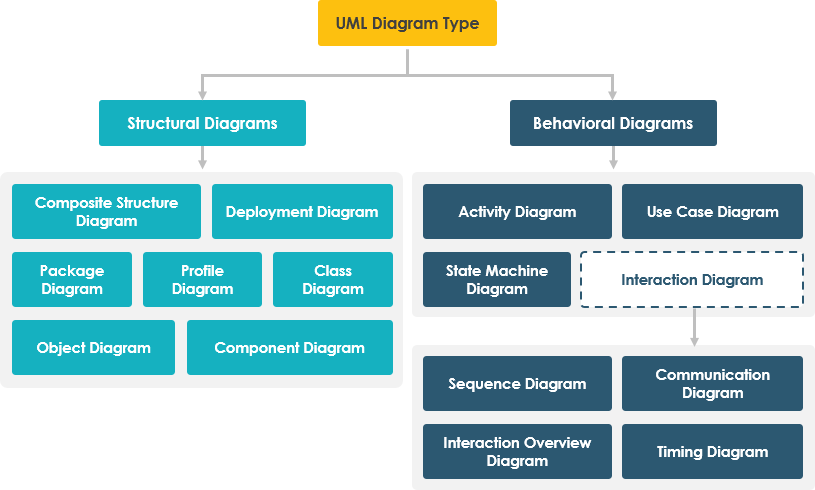
\includegraphics[width=1.0\linewidth]{01-uml-diagram-types.png}
    \caption{A map of the 14 UML diagram types, grouped into their respective categories, with an additional breakdown of the interaction diagrams subcategory\cite{visualpara}.}
    \label{fig:UML Diagram Map}
\end{figure}

\subsubsubsection{Sequence Diagram}

Sequence diagrams belong to a sub-category of interaction diagrams, which includes communication, timing, and interaction overview diagrams\cite{Seidl_Scholz_Huemer_Kappel_Duffy_2014}.

Sequence diagrams model communication protocols between human and non-human entities. The horizontal axis represents the sequence of communication messages, while the vertical axis shows the timing of interactions. Each element in a sequence diagram is represented by a lifeline extending vertically, which may terminate if it is no longer required in the system. Messages are represented by arrows connecting elements at various stages of their lifecycle. 

Figure 2 presents a simplified sequence diagram that expands on the earlier analogy of a \texttt{Human} class. In this example, the \texttt{person} instances are depicted as human actors interacting with each other and a non-human \texttt{mirror} object in a system.

\begin{figure}[H]
    \centering
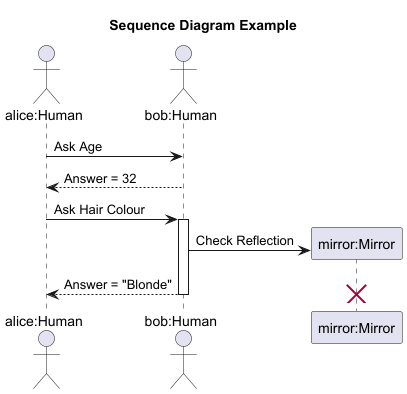
\includegraphics[width=0.7\linewidth]{SDexample-Sequence_Diagram_Example.png}
    \caption{A simple sequence diagram: Alice asks Bob his age and receives the reply "32". Bob consults a non-human "mirror" object to answer the second query, and the mirror's lifeline terminates once it is no longer needed.}
    \label{fig:Simple SD}
\end{figure}

\subsubsubsection{Class Diagram}

The class diagram defines the structure of classes within a system\cite{Seidl_Scholz_Huemer_Kappel_Duffy_2014}. Each class is depicted as a rectangular element containing information about the attributes it holds and the operations it can perform. Interconnected edges represent the associations between different classes in the system, defining their specific relationships and interactions. The class diagram provides an overview of the modelled system's structural architecture. Figure 3 continues with the \texttt{Human} class analogy to give a simplified class diagram.

\begin{figure}[H]
    \centering
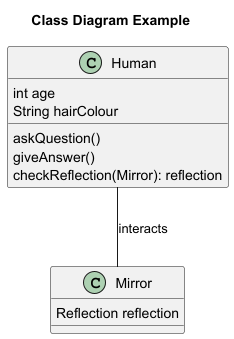
\includegraphics[width=0.4\linewidth]{CDexample-Class_Diagram_Example.png}
    \caption{A simple class diagram: The \texttt{Human} class has attributes \texttt{age} and \texttt{hairColour} and can perform the operations \texttt{askQuestion()}, \texttt{giveAnswer()}, and \texttt{checkReflection()} if given a mirror. It has an "interacts" association with a \texttt{Mirror} class, which returns its \texttt{reflection} attribute when \texttt{checkReflection()} is called.}
    \label{fig:Simple CD}
    \end{figure}

\subsubsubsection{Profile Diagram}

The profile diagram is another structural diagram used to modify general-purpose UML diagrams to become domain-specific.

The composition of a UML diagram is modelled using UML itself. Class diagrams illustrate the structure of each of the fourteen UML diagram types, including their own structure. Together, these class diagrams form the UML meta-model\cite{Seidl_Scholz_Huemer_Kappel_Duffy_2014}.

There are three methods for tailoring the UML meta-model to a specific domain, with the appropriate approach chosen based on the required level of specificity. These methods, in order of decreasing intensity, are creating an entirely new meta-model for the domain, modifying the existing UML meta-model by introducing new meta-classes and meta-associations or leveraging UML's built-in extension mechanism—the UML profile diagram\cite{Seidl_Scholz_Huemer_Kappel_Duffy_2014}.

The profile diagram uses stereotypes, a type of meta-class, to modify existing meta-classes in the meta-model. For example, the meta-classes \textbf{Association} and \textbf{Class} are part of the class diagram meta-model, while \textbf{Message} and \textbf{Lifeline} are used in the sequence diagram meta-model. Stereotypes are denoted by the tag \texttt{<<Stereotype>>}, followed by their name. These stereotypes are connected to the meta-classes they modify through an extension relationship pointing from the stereotype to the meta-class it's modifying\cite{Seidl_Scholz_Huemer_Kappel_Duffy_2014}.

A stereotype can include meta-attributes or carry a note. Notes typically provide additional context or clarification in natural language. The stereotype name, meta-attributes, and notes impose constraints on the meta-class being extended, thus refining the system's structure and behaviour by introducing domain-specific constraints\cite{Seidl_Scholz_Huemer_Kappel_Duffy_2014}. 

Figure 4 illustrates how a profile diagram, tailored to an academic domain, constrains the class diagram meta-model by applying stereotypes to its meta-classes. Figure 5 showcases the integration of this profile diagram into a class diagram's design through the use of stereotype tags.

\begin{figure}[H]
    \centering
    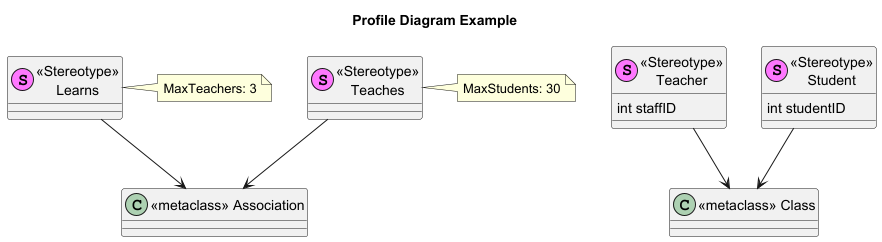
\includegraphics[width=1\linewidth]{PDExample-Profile_Diagram_Example.png}
    \caption{A simple profile diagram applied to the class diagram meta-model. The stereotypes \texttt{<<Teacher>>} and \texttt{<<Student>>} are applied to classes, each containing meta-attributes related to their respective IDs. The stereotypes \texttt{Learns} and \texttt{Teaches} are assigned to associations, with notes specifying limits on how many "teaches" or "learns" associations can exist within a system.}
    \label{fig:Simple PD 1}
\end{figure}

\begin{figure}[H]
    \centering
    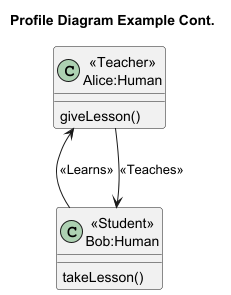
\includegraphics[width=0.3\linewidth]{PDExample2.png}
    \caption{A class diagram implementing the profile diagram stereotypes. Classes and associations are tagged with their respective stereotypes, inheriting the constraints defined in Figure 4.}
    \label{fig:Simple PD 2}
\end{figure}

\subsubsection{Q-SE 2021}

The second Q-SE workshop held virtually in June 2021 included a segment focused on modelling quantum systems\cite{QSE2021}. During this session, Luis Jiménez-Navajas presented the paper \textit{"Modelling Quantum Circuits with UML"}\cite{Pérez-Castillo2021}, co-authored with Ricardo Pérez-Castillo and Mario Piattini. The paper introduced the concept of creating a UML profile diagram that could incorporate a quantum domain, using the example of an activity diagram to model a quantum circuit\cite{Pérez-Castillo2021}. 

Pérez-Castillo and Piattini further expanded on this work and, in 2022, published the paper \textit{"Design of Classical-Quantum Systems with UML"}\cite{Pérez-Castillo2022} in the Springer May 2022 \textit{Computing} journal\cite{Computing2022}. They also served as editors for \textit{“Quantum Software Engineering”}\cite{serrano2022quantum}, also published by Springer, which included a revision of Pérez-Delgado's Q-UML work. The follow-up paper, \textit{“A Quantum Software Modeling Language”}\cite{Pérez-Delgado2022}, further developed Q-UML by introducing additional pictorial elements for modelling quantum components and establishing a fundamental axiom and five core design principles.

Pérez-Castillo et al. built upon earlier efforts to develop a quantum UML profile diagram by extending its application to multiple UML diagram types. 

Pérez-Delgado's work with Q-UML modelled Shor's algorithm in the context of a quantum computer exhibiting quantum advantage, while Pérez-Castillo et al. modelled hybrid information systems. These hybrid systems, which combine classical and quantum processors, are already operational and can be executed on existing quantum hardware.

\subsubsection{NISQ}

As the introduction mentions, classical and quantum computers differ fundamentally in their underlying hardware. Classical computers operate in a binary, deterministic state where bits are clearly defined as 0 or 1. In contrast, quantum computers leverage the principles of quantum mechanics, using qubits instead of bits. A qubit can exist in a superposition of 0 and 1, with its final state determined probabilistically when measured. 

The ability for qubits to exist in superpositions allows quantum computers to accelerate the speed at which certain types of problems can be solved \cite{NielsenChuang2010}. A well-known example is factoring large prime numbers, a computational task that classical computers find difficult to solve within a reasonable time frame. Peter Shor’s development of Shor’s algorithm demonstrates how a sufficiently powerful quantum computer could theoretically perform prime factorisation significantly faster than its classical counterpart\cite{Shor_1997}\cite{minutephysics}. The Rivest-Shamir-Adleman (RSA) encryption algorithm is a widely used encryption protocol which relies on classical computers' difficulty in factoring large prime numbers\cite{encryptionconsulting}. A powerful enough quantum computer could pose a risk to modern-day security protocols as we currently know them. 

Quantum computing aspires to reach the same level of ubiquity as classical computing while achieving quantum supremacy and quantum advantage. Quantum supremacy would enable quantum computers to solve tasks that classical computers cannot complete within a reasonable time frame, such as factorisation of large prime numbers\cite{quera}. Quantum advantage would allow quantum systems to solve real-world problems \textit{"faster than any classical algorithm running on any classical computer"}\cite{quera}. To reach this point, quantum computers must scale up the number of qubits required for complex calculations—a critical challenge they face today.

Qubits are susceptible to environmental decoherence and noise, which can lead to errors and affect their ability to retain their quantum state\cite{Preskill2018}. Despite notable progress in increasing qubit counts, significantly more qubits are needed to enable error-correction methods for fault-tolerant quantum computing required for quantum advantage and quantum supremacy\cite{Willsch2022}.

The Noisy Intermediate-Scale Quantum (NISQ) era refers to hardware with qubit counts ranging from tens to hundreds\cite{Preskill2018}. This technology is currently available, with IBM's Qiskit Runtime Service as an example of NISQ hardware utilisation\cite{ReleaseSummary}. Despite their limited qubit capacity, these systems support computations through hybrid algorithms that leverage quantum and classical resources. One such algorithm is the Variational Quantum Eigensolver.

\subsubsection{VQE}

VQE is a hybrid quantum-classical algorithm that can find the ground state, the lowest energy, of a given physical system\cite{Tilly2022}. VQE can aid in quantum chemistry simulations where determining the ground state of a given molecule or atom \textit{"provides essential information about the system's stability, reactivity, and other chemical properties"}\cite{queragroundstate}. VQE has many potential applications but can be considered a viable candidate for optimisation problems; it can be used to find a global or best local minimum (or maximum) solution within a search space\cite{vqeqiskit}\cite{VQEMax}. 

VQE belongs to a class of near-term algorithms designed to run on NISQ devices. As the depth of a quantum circuit increases, error rates also rise due to decoherence, requiring more qubits for error correction. Near-term algorithms seek techniques for solving non-trivial problems using limited qubit count whilst negating decoherence\cite{Huang_2023}. VQE uses a shallow quantum circuit and delegates tasks between the quantum circuit and a classical optimiser to find its solution\cite{vqeqiskit}\cite{Peruzzo2014}.

The VQE algorithm contains the following core components:

\textbf{Hamiltonian} - A matrix that represents the total energy of a physical system\cite{hamiltonian}. The eigenvalues of the Hamiltonian correspond to the system's energy levels, with the lowest eigenvalue representing the system's ground state\cite{vqeqiskit}.

\textbf{Ansatz} - A trial state for the Hamiltonian that represents an educated guess for finding the Hamiltonian's approximate ground state. The ansatz is a parametrised quantum circuit, with its parameters iteratively updated and the energy estimate evaluated against the Hamiltonian to find the lowest energy estimate\cite{Tilly2022}\cite{Tutorial}.

\textbf{Cost Function} - A function that defines the objective of the problem, whether it involves minimisation or maximisation\cite{vqeqiskit}.

\textbf{Optimiser} - A classical optimiser that evaluates the output of the ansatz and iteratively adjusts its parameters, seeking to find the optimal set of parameters for the problem solution\cite{Tutorial}\cite{vqeqiskit}. 

The pseudocode for the VQE algorithm is as follows:

\begin{algorithm}[H]
\caption{Variational Quantum Eigensolver (VQE)}\label{vqe_algorithm}
\begin{algorithmic}[1]
\State Define Hamiltonian \( \mathcal{H} \)
\State Prepare ansatz \( \mathcal{A} \) with \( k \) parameters \( \overrightarrow{\theta} \)
\State Define cost function $\mathcal{C}$ as either minimisation ($\bigwedge$) or maximisation ($\bigvee$)
\State Initialise a classical optimizer \( O \)
\While{convergence criterion not met and max iterations not exceeded}
    \State Calculate expectation value \( E \) by evaluating \( \mathcal{A}(\overrightarrow{\theta}) \) with \( \mathcal{H} \)
    \State Update \( \overrightarrow{\theta} \) using \( O \) to optimise \( E \)
\EndWhile
\State \Return optimal parameters \( \overrightarrow{\theta} \) and solution \( E \)
\end{algorithmic}
\end{algorithm}

The VQE algorithm can be implemented and executed using quantum programming languages, with IBM’s Qiskit being a popular choice.

\subsubsection{Qiskit}

Qiskit is an open-source software development kit (SDK) created by IBM to access and utilise their cloud-based quantum computing services. Written in Python, Qiskit provides tools and libraries for quantum programming, simulation, and experimentation\cite{qiskithomepage}.

IBM Quantum Learning offers online tutorials that guide users through implementing quantum algorithms with the Qiskit SDK\cite{Tutorial}. The UML diagrams created for this paper are based on the IBM tutorial demonstrating the VQE algorithm in Qiskit\cite{IBMVQETut}.

\subsubsubsection{Qiskit and VQE}

This section provides a comprehensive overview of the specific implementation of VQE as outlined in the Qiskit IBM tutorial. It aims to offer a clear understanding of the associated UML diagrams. The tutorial's code is included in the appendix for reference.

The instance \textbf{hamiltonian} is initialised from the class \textbf{SparsePauliOp} by calling the \textit{.from\_list()} method in its construction. The \textbf{hamiltonian} object is a classical representation of Pauli operators, where each operator is given as a string (e.g., "X", "Y", "Z", or "I" for identity). Pauli operators are 2×2 matrices corresponding to spin measurements along the x, y, and z axes\cite{DJORDJEVIC201229}. Each operator string specifies actions on individual qubits. The VQE tutorial uses a 2-qubit system, acting on pairs of Pauli strings referred to as operator terms. The tensor product of these pairs is assigned a coefficient that defines the strength of each operator term. The linear combination of these terms represents the system's total energy, the Hamiltonian. Only non-zero operator terms and coefficients are stored, resulting in a sparse representation of the Hamiltonian to reduce computational expense\cite{EITCA2024}\cite{SparsePauliOp}\cite{PauliList}.

The instance \textbf{ansatz} is initialised from the class \textbf{EfficientSU2} with the number of qubits \textbf{hamiltonian} holds passed to it in its construction. The \textbf{EfficientSU2} class provides a hardware-efficient classical representation of a quantum circuit\cite{EfficientSU2}. The circuit comprises layers of single-qubit operations (such as Pauli rotation gates) and C-NOT gates, which entangle the qubits\cite{EfficientSU2}. Each operation holds a parameter which will be iteratively adjusted to find the lowest energy state.

The instance \textbf{backend} is initialised from the class \textbf{QiskitRuntimeService}. The \textbf{QiskitRuntimeService} class interacts with the IBM Qiskit Runtime Service that provides access to quantum hardware and quantum simulators. The parameter \textbf{ibm\_quantum} is given to \textbf{backend} during its construction to connect through an IBM quantum account\cite{qrsreadme}. The method \textit{least.busy()} is used to select the next available quantum hardware with the parameter \textbf{simulator} set to false.

\textbf{QiskitRuntimeService} will instantiate an \textbf{IBMBackend} object. The attribute \textbf{target} of the \textbf{IBMBackend} object is accessed and passed as a parameter to the instance \textbf{pm} of the \textbf{StagedPassManager} class, created using the \textit{generate\_preset\_pass\_manager()} method. This process allows the pass manager to receive information regarding the constraints of the selected quantum hardware.

The pass manager will \textit{"define a typical full compilation pipeline from an abstract virtual circuit to one that is optimized and capable of running on the specified backend"}\cite{StagedPassManager}. The \textit{.run()} method is executed on \textbf{pm} to transform \textbf{ansatz} to be compatible with the selected quantum hardware's instruction set architecture (ISA), with the newly transformed ansatz stored in a new variable \textbf{ansatz\_isa}\cite{ISACirc}. The \textit{.apply\_layout()} method is then called on \textbf{hamiltonian}, with \textbf{ansatz\_isa} passed as a parameter, to modify its layout to be compatible with the selected quantum hardware ISA. The modified Hamiltonian is then stored as a new variable  \textbf{hamiltonian\_isa}.

The cost function method \textbf{cost\_func} is a user-defined function that facilitates access to the quantum hardware and will obtain an approximate energy estimate of the Hamiltonian. It accepts an estimator and the components of a primitive unified bloc (PUB) as its parameters. 

 Qiskit offers two primary primitives—"Estimator" and "Sampler"—designed to simplify foundational quantum tasks\cite{QiskitRuntime}. Estimator primitives \textit{"accept combinations of circuits and observables ... to estimate expectation values of the observables"}\cite{Primitives}. The estimator accepts the quantum circuit \textbf{ansatz\_isa} and the observable \textbf{hamiltonian\_isa} to produce an estimated expectation value of the Hamiltonian's energy. The estimator is defined later in the code, created by the class \textbf{EstimatorV2}. The PUB is the input given to the estimator primitive.

PUB comprises of an array of initial guesses for the parameters of the ansatz, the \textbf{hamiltonian\_isa} given as a list, and the quantum circuit \textbf{ansatz\_isa}. These components form a tuple and are assigned to the variable \textbf{pub}, which is given as a parameter for the estimator object's \textit{.run()} method. 

When \textit{estimator.run()} is executed, the classical, parametrised \textbf{ansatz\_isa} circuit is transpiled into a quantum circuit that is compatible with the selected quantum hardware. It is then executed on the quantum computer, preparing a quantum state based on its current parameters\cite{EstimatorV2}\cite{Tutorial}. The \textbf{hamiltonian\_isa} list, which represents the system's Hamiltonian, is applied to this prepared quantum state. This guides the estimator in computing the energy expectation value of the system being modelled through the \textbf{ansatz\_isa} circuit. Once the operation is complete, the \textit{.result()} method returns a container of PUB results\cite{PrimitiveResult}, with slicing used to access the estimated energy of the \textbf{ansatz\_isa}, which is stored in the variable \textbf{energy}.

A dictionary named \textbf{cost\_history\_dict} stores the parameter, iteration, and energy estimate each time the estimator's \textit{.run()} method is executed. Its initial values consist of a placeholder for the parameters, iteration set to zero and an empty list for the energy estimate, with each energy estimate being appended to the list per execution. 

Finally, \textbf{cost\_func} returns the value of the \textbf{energy} variable as its result after being called.

A random array of initial guess parameters, assigned to the variable \textbf{x0}, is constructed using NumPy’s constant $\pi$ and its \textit{random.random()} method. The code generates an array of random floating-point numbers, scaled to the range of [0,$\pi$2], to account for every quantum state that can be represented on the Bloch sphere (a geometrical, spherical representation of a qubits state space\cite{blocsphere}). The \textbf{ansatz} attribute \textbf{num\_parameters} sets the size of the array, having been stored earlier in the variable \textbf{num\_params}, to match the number of parameters to assign to each of operations in the ansatz circuit. The \textbf{x0} array will be given to \textbf{cost\_func} as the parameters required for the \textbf{pub} variable and updated iteratively to find the set of parameters that produce the lowest energy estimate of the system.

The instance \textbf{session} is initialised from the class \textbf{Session} with \textbf{backend} passed as a parameter to configure it to the selected quantum hardware. The instance \textbf{estimator} is then initialised from the class \textbf{EstimatorV2} with \textbf{session} passed to the estimator's \textbf{mode} attribute. This estimator, which operates within \textbf{cost\_func}, uses \textbf{session} to execute computations on the specified quantum backend. Assigning a  \textbf{Session} object as the estimator's \textbf{mode} facilitates the grouping of iterative calls to the quantum computer when \textit{estimator.run()} executes, efficiently managing the allocation of jobs to quantum resources\cite{Session}.

The instance \textbf{res} of the classical \textbf{Minimize} class from the SciPy package is initialised with the Constrained Optimization by Linear Approximation (COBYLA) method, which is used to minimise a scalar function\cite{Minimize}. In this case, the scalar function is the \textbf{cost\_func} method, which returns a scalar energy estimate as a float. The parameters for \textbf{res} include the \textbf{cost\_func} and a tuple which contains the objects that need to be passed to the cost functions parameters; \textbf{x0}, \textbf{ansatz\_isa}, \textbf{hamiltonian\_isa}, and \textbf{estimator}.

During the optimisation loop, \textbf{cost\_func} calculates and returns the energy estimate of \textbf{ansatz\_isa}, while \textbf{res} iteratively updates the parameters in \textbf{x0}, adjusting the ansatz's parameters to minimize the energy estimate. Each call to \textbf{cost\_func} invokes the \textit{estimator.run()} method and performs 10,000 shots on the quantum circuit before returning the energy estimate. The loop continues until the energy estimate converges to the lowest achievable value, representing the ground-state energy\cite{Tutorial}.

Upon completion of the optimisation loop, successful termination of the process is verified by comparing the solution parameter and evaluation count against the stored solution parameter and iteration count within \textbf{cost\_history\_dict} maintained by the \textbf{cost\_func} method. These results are then visualised using the matplotlib package, plotting a graph with the number of iterations on the x-axis and the energy estimates on the y-axis.

\subsection{Related Work}

\subsubsection{Q-UML}

The paper \textit{"A Quantum Software Modeling Language"} highlights the significant role modelling languages have played in enabling professionals from diverse disciplines to advance classical software engineering. This collaboration has been instrumental in making classical computers a ubiquitous part of modern life. Pérez-Delgado argues that while modelling large-scale quantum systems is not a pressing need, the introduction of a quantum modelling language could act as an \textit{intuition pump}, accelerating the development of quantum software engineering to achieve the maturity and integration of its classical counterpart\cite{Pérez-Delgado2022}.

Pérez-Delgado defines one fundamental axiom and five core design principles when constructing a quantum software modelling language. 

The fundamental axiom is that \textit{"quantum software
engineering should be as similar to classical software engineering as possible, but no more"}\cite{Pérez-Delgado2022}. A quantum modelling language must allow professionals familiar with classical software modelling techniques to adapt to its notation quickly. It must also clearly differentiate between its classical and quantum components as they handle fundamentally different types of information: \textit{"Quantum information can be put in superposition, classical information
cannot. Classical information can be cloned or copied, quantum information—in
general—cannot"}\cite{Pérez-Delgado2022}.

The five core design principles establish when and how classical and quantum elements must be differentiated in a quantum modelling language. They are explained as follows: 

\textbf{Quantum Classes}: If a class/object needs to use quantum information in its design or interactions, it must be labelled quantum.

\textbf{Quantum Elements}: Operations and attributes must be defined as either classical or quantum. The data types of variables must be labelled. The input and output of operations must be labelled. 

\textbf{Quantum Supremacy}: If an object does not use any quantum information for its design, interactions or relationships with other objects, it will always remain classical. It will be upgraded to quantum when it requires even one quantum element. 

\textbf{Quantum Aggregation}: An object composed of at least one other quantum object will be labelled as quantum.

\textbf{Quantum Communication}: Quantum and classical objects can communicate with each other if the message can be translated from quantum information to classical information. Quantum and classical messages must be labelled.

The axioms and design principles are culminated and applied to the UML extension Q-UML, with the paper providing examples of its implementation by example of a use case, class, state, activity, and sequence diagram modelling Shor's algorithm\cite{Pérez-Delgado2022}. Q-UML uses bold text and double lines to distinguish quantum elements in the diagram. Sections 3.4.1 and 3.5.1 delve deeper into the methodology for applying Q-UML to sequence and class diagrams.

\subsubsection{Quantum UML Profile}

The paper \textit{"Design of Classical-Quantum Systems with UML"} presents a quantum UML profile designed to address the gap in analysis and design techniques for hybrid classical-quantum information systems\cite{Pérez-Castillo2022}. 

Pérez-Castillo et al. highlights two main challenges in the development of quantum software practices: first, the ad-hoc approach to quantum programming languages, which is often \textit{"without any prior design or modelling"}\cite{Pérez-Castillo2022}, and second, the necessity for classical and quantum information systems to be \textit{"analysed and designed together"}\cite{Pérez-Castillo2022}. 

The authors argue that classical computers will not be replaced by quantum computers, as classical machines are still more cost-effective for many tasks. Instead, classical computers will serve as coordinators, managing requests to quantum software systems\cite{Pérez-Castillo2022}. This highlights the importance of developing design documentation that accommodates classical and quantum computing systems and outlines their interactions for design and analysis.

Pérez-Castillo et al. present UML as a viable tool for modelling hybrid quantum-classical systems. They reference Pérez-Delgado's Q-UML as an existing approach to modifying UML but classify it as a Domain-Specific Language (DSL) rather than a valid UML extension\cite{Pérez-Castillo2022}}. This distinction arises because Q-UML employs specific notations, such as double lines and bold text, which do not conform to the official UML standard. In contrast, the UML quantum profile diagrams outlined in the paper are UML-compliant, adhering to the existing UML specifications\cite{Pérez-Castillo2022}. 

Pérez-Castillo et al. introduce a UML profile for various UML diagram types, including use case, class, sequence, activity, and deployment diagrams. This paper focuses on the class and sequence UML profile diagrams applied to the UML models discussed in sections 3.4.2 and 3.5.2.

\subsubsubsection{Class Diagram Meta-Model}

The class diagram meta-model contains the stereotypes \texttt{<<Quantum>>}, \texttt{<<Quantum Driver>>}, and \texttt{<<Quantum Request>>}.

The \texttt{<<Quantum>>} stereotype constrains the meta-classes \textbf{Package} and \textbf{Class}. It is used to model classes and packages that enable quantum functionality such as \textit{"quantum
circuits, algorithms, or similar artefacts"}\cite{Pérez-Castillo2022}.

The \texttt{<<Quantum Driver>>} stereotype constrains the \textbf{Class} meta-class. It is used to model classes that manage communication with quantum software\cite{Pérez-Castillo2022}. 

The \texttt{<<Quantum Request>>} stereotype constrains the meta-classes \textbf{AssociationClass}, \textbf{Class}, \textbf{Dependency}, and \textbf{Operation}. It is an optional modelling choice used to represent calls from a \texttt{<<Quantum Driver>>} to a \texttt{<<Quantum>>} class, linking associated elements involved in the communication, such as cost functions and classical optimisers. It can also be used to model quantum operations within a class\cite{Pérez-Castillo2022}.

Figure 6 shows the class diagram meta-model with the application of the quantum UML profile extensions.

\begin{figure}
    \centering
    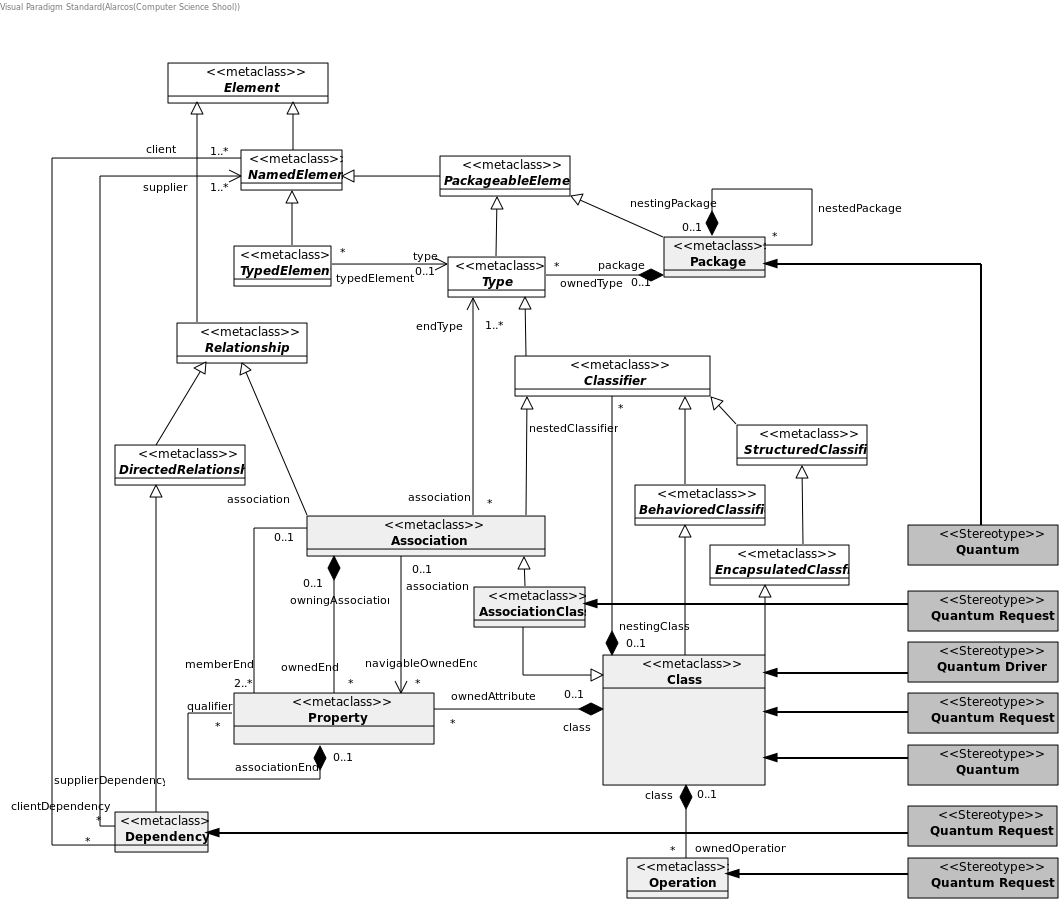
\includegraphics[width=1\linewidth]{QuantumUMLProfile-ClassDiagram.png}
    \caption{The quantum UML profile applied to the class diagram meta-model\cite{PerezCastillo2021Git}.}
    \label{fig:QUMLPD_CD}
\end{figure}

\subsubsubsection{Sequence Diagram Meta-Model}

The sequence diagram meta-model contains the stereotypes \texttt{<<Quantum Driver>>}, \texttt{<<Quantum>>}, \texttt{<<Quantum Request>>}, \texttt{<<Quantum Reply>>}, and \\ \texttt{<<Quantum Computer>>}.

The \texttt{<<Quantum Driver>>} and \texttt{<<Quantum>>} stereotypes both constrain the \textbf{Lifeline} meta-class. They align with the definitions established in the class diagram meta-model: \texttt{<<Quantum Driver>>} represents elements that enable communication with quantum software. The \texttt{<<Quantum>>} stereotype represents elements that provide quantum functionality.

The \texttt{<<Quantum Request>>} stereotype constrains the meta-class \textbf{Lifeline}, modelling elements created or linked by the call between a \texttt{<<Quantum Driver>>} and a \texttt{<<Quantum>>} element\cite{Pérez-Castillo2022}.

The \texttt{<<Quantum Request>>} and \texttt{<<Quantum Reply>>} stereotypes constrain the meta-class \textbf{Message}, modelling communications that either send or receive quantum information\cite{Pérez-Castillo2022}.

The \texttt{<<Quantum Computer>>} stereotype constrains the meta-class \textbf{Actor}, which denotes quantum machines if modelled in the diagram.

Figure 7 shows the sequence diagram meta-model with the application of the quantum UML profile extensions.

\begin{figure}
    \centering
    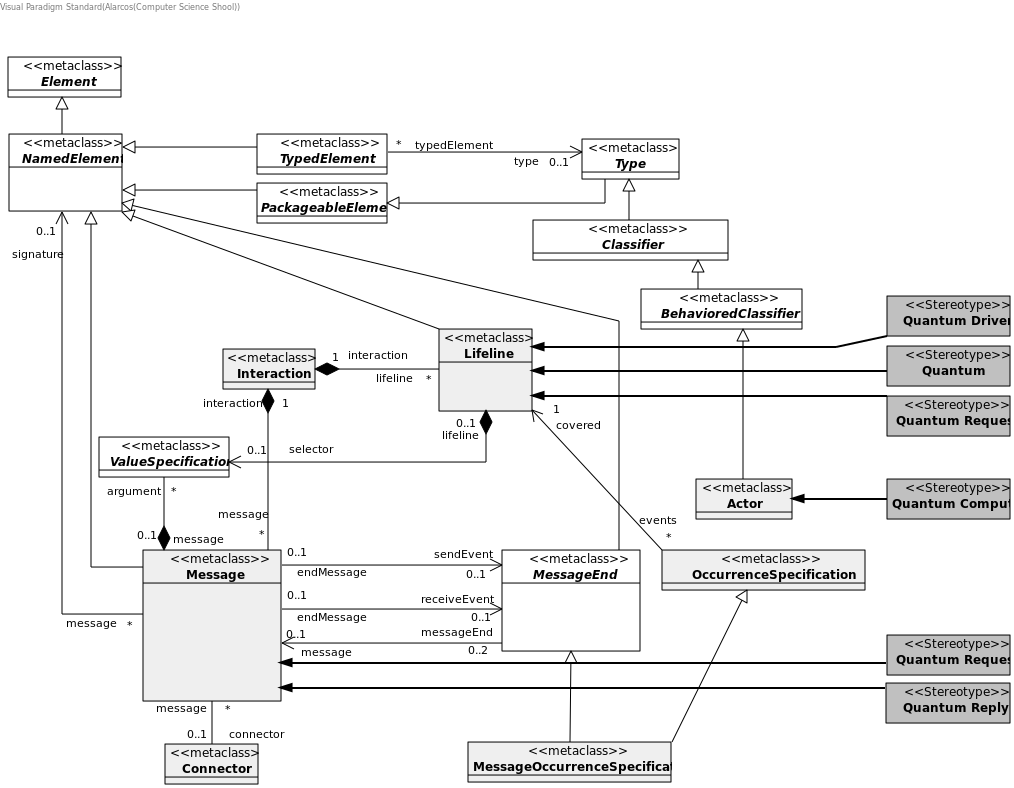
\includegraphics[width=1\linewidth]{QuantumUMLProfile-SequenceDiagram.png}
    \caption{The quantum UML profile applied to the sequence diagram meta-model\cite{PerezCastillo2021Git}.}
    \label{fig:QUMLPD_SD}
\end{figure}

\section{Design and Implementation}

This section details the creation of UML sequence and class diagrams used to model the VQE algorithm, as implemented on IBM's Quantum Learning platform\cite{IBMVQETut}. It begins with an overview of the tools employed for diagram creation and why they were chosen, followed by a step-by-step breakdown of the diagram construction process. General notation conventions for all diagrams are outlined first, followed by a detailed explanation of how the VQE algorithm is represented in the sequence diagram. Subsequent sections explore how these diagrams are adapted into the Q-UML and quantum UML profile formats. The same approach is then applied to the VQE class diagrams.

\subsection{Plant UML}

During this project's research and development phase, numerous online tools for diagram construction were explored. Text-to-graphic tools were selected for their accessible format, allowing the creation of UML-compliant diagrams through straightforward scripting. PlantUML, one of the most well-known and established versions of these text-to-graphic tools, was chosen as the primary tool for drafting the initial diagrams.

PlantUML is an open-source tool for creating various diagram types, including UML. It enables users to generate diagrams using plain text descriptions, which are then rendered into a graphical output\cite{PUML}.

\subsection{Lucidchart}

Lucidchart is a web-based application that supports the creation of various diagrams, including UML. It offers a graphical user interface(GUI) for customisation and flexibility. To accommodate the Q-UML adaptations—such as the double-lined pictorial elements, which are not natively supported in PlantUML—the diagrams originally drafted in PlantUML were replicated in Lucidchart. This allowed for the necessary visual modifications and ensured consistency in comparison across both diagram adaptations.

\subsection{UML Design Choice}

UML offers users flexibility in choosing the level of detail required to represent system information within a diagram. It is essential to strike a balance between including sufficient information for clarity and avoiding over-complication, as UML diagrams should provide a high-level abstraction of the system. This section outlines the general formatting principles applied to all UML diagrams in this project. Subsequent sections on the VQE sequence and class diagrams will delve into specific design choices and their underlying rationale. Much of the reference material for constructing these diagrams has been sourced from the book \textit{UML @ Classroom}\cite{Seidl_Scholz_Huemer_Kappel_Duffy_2014}. 

All UML diagrams consist of a content area populated by boxes and edges, which together form the specific design of each diagram type. An optional framing element was included in the UML diagrams for this project, enclosing these components within a boundary. The frame header displays the namespace of the system the diagram represents\cite{OMG_UML}. For this project, the namespace "Variational Quantum Eigensolver" is used, with abbreviations indicating the type of diagram preceding it. 

\subsection{VQE Sequence Diagram}

The elements in the sequence diagram represent the instances of classes in the IBM VQE Qiskit tutorial. Each instance is depicted as a rectangle, with a dashed, vertical lifeline extending downward from its creation to connect to a duplicated element at the bottom of the frame, where all the system elements are aligned. The naming convention follows the format \textit{instance:Class}.

Message sequences are simplified where possible to illustrate the provision of an attribute from one instance to another or to illustrate an operation's execution. For example, the message \textit{.num\_qubits} passed from the \textbf{hamiltonian} to the \textbf{ansatz} could have been a sequence of messages where the \textbf{ansatz} first requests the \textbf{.num\_qubits} attribute from the \textbf{hamiltonian} and the \textbf{hamiltonian} provides it as a response message, depicted by a dashed line and open arrowhead. This is more accurate; however, it would result in an over-complicated diagram of many messages. 

All messages in the diagram are synchronous, pointing from a sender to a receiver. A synchronous message indicates that the message must be received before the sender can continue with any further instructions\cite{Seidl_Scholz_Huemer_Kappel_Duffy_2014}. For example, the instance \textbf{pm:PassManager} cannot execute its \textit{pm.run(ansatz)} message until \textbf{backend:QiskitRuntimeService} passes its constraints and optimisation level. A continuous line and a filled triangular arrowhead depict a synchronous message.

The \textbf{IBMBackend} element was omitted from the sequence diagram, opting instead to show messages invoking this object as originating from \textbf{backend:QiskitRuntimeService}.
The naming convention effectively conveys that \textbf{QiskitRuntimeService} serves as a "backend" instance. Adding \textbf{IBMBackend} would introduce unnecessary complexity to the sequence diagram, where the emphasis is on message flow rather than object details. These specifics are more appropriately captured in the class diagram, where \textbf{IBMBackend} has been included.

The transformation of \textbf{hamiltonian} and \textbf{ansatz} to \textbf{hamiltonian\_isa} and \textbf{ansatz\_isa} is depicted by a destruction event; a red cross on the lifeline at the point where \textbf{hamiltonian} and \textbf{ansatz} are no longer used in the system.

Activation bars are slim, vertical rectangles that overlay an element's lifeline,  representing a process that involves multiple elements for its execution\cite{Seidl_Scholz_Huemer_Kappel_Duffy_2014}. This occurs when \textbf{pm} executes its \textit{run()} method, \textbf{hamiltonian} executes \textit{apply\_layout(layout=ansatz\_isa.layout)}, and the execution of both \textbf{cost\_func} and \textbf{res}.

The diagram uses two \textit{loop} fragments and an \textit{alt} fragment. The loop fragment expresses a sequence that is repeatedly executed, with a boundary encompassing the messages involved in the repeated sequence\cite{Seidl_Scholz_Huemer_Kappel_Duffy_2014}. An outer loop contains the repeated exchange of messages between \textbf{cost\_func} and \textbf{res} as they seek to find the lowest energy estimate. An inner loop contains the repeated runs of the quantum circuit when \textit{estimator.run()} is executed. The upper right corner of the fragment includes a heading of the fragments label and a description of how long the process executes; the outer loop running until \textbf{[lowest energy estimate found]} and the inner loop running \textbf{[10,000 shots]}. The response message from the estimator is shown outside of this loop, as it does not return a result after each shot but once the circuit has completed 10,000 shots. 

The alt fragment in UML represents alternative sequences\cite{Seidl_Scholz_Huemer_Kappel_Duffy_2014}. Here, it evaluates whether the results of the \textbf{cost\_history\_dict} match those from the completed minimisation routine. A true or false boolean outcome determines whether the verification is successful or unsuccessful.

\subsubsection{SD QUML}

The elements \textbf{backend}, \textbf{estimator} and \textbf{cost\_func} are depicted as quantum through the use of bold text for their names, double lines for their rectangle elements and double lines for their lifelines. 

The instance \textbf{backend} facilitates communication between quantum and classical machines. Although the messages it sends in the diagram remain classical, the design of the class from which it is called, \textbf{QiskitRuntimeService}, is fundamentally quantum as it manages interactions with quantum hardware, following the first design principle \textbf{Quantum Classes}. The \textbf{estimator} element is also the instance of a quantum class that executes the ansatz circuit through its \textit{.run()} operation. The \textbf{cost\_func} element contains \textbf{estimator} in its design and is a user-defined class in the context of this model. It, therefore, also follows the first design principle. 

The sequence diagram includes one quantum message: \textbf{cost\_func} sends a request to \textbf{estimator} invoking its \textit{.run()} method. This request triggers \textbf{estimator} to access quantum hardware and compute the energy estimate using quantum information based on the current parameters. The quantum nature of this message is denoted using double lines for the synchronous message, with the message details displayed in bold text. The reply message from \textbf{estimator} remains classical as the results are converted to classical information before being returned to \textbf{cost\_func}.

The corresponding diagram is presented in Figure 8.

\begin{sidewaysfigure}
    \centering
    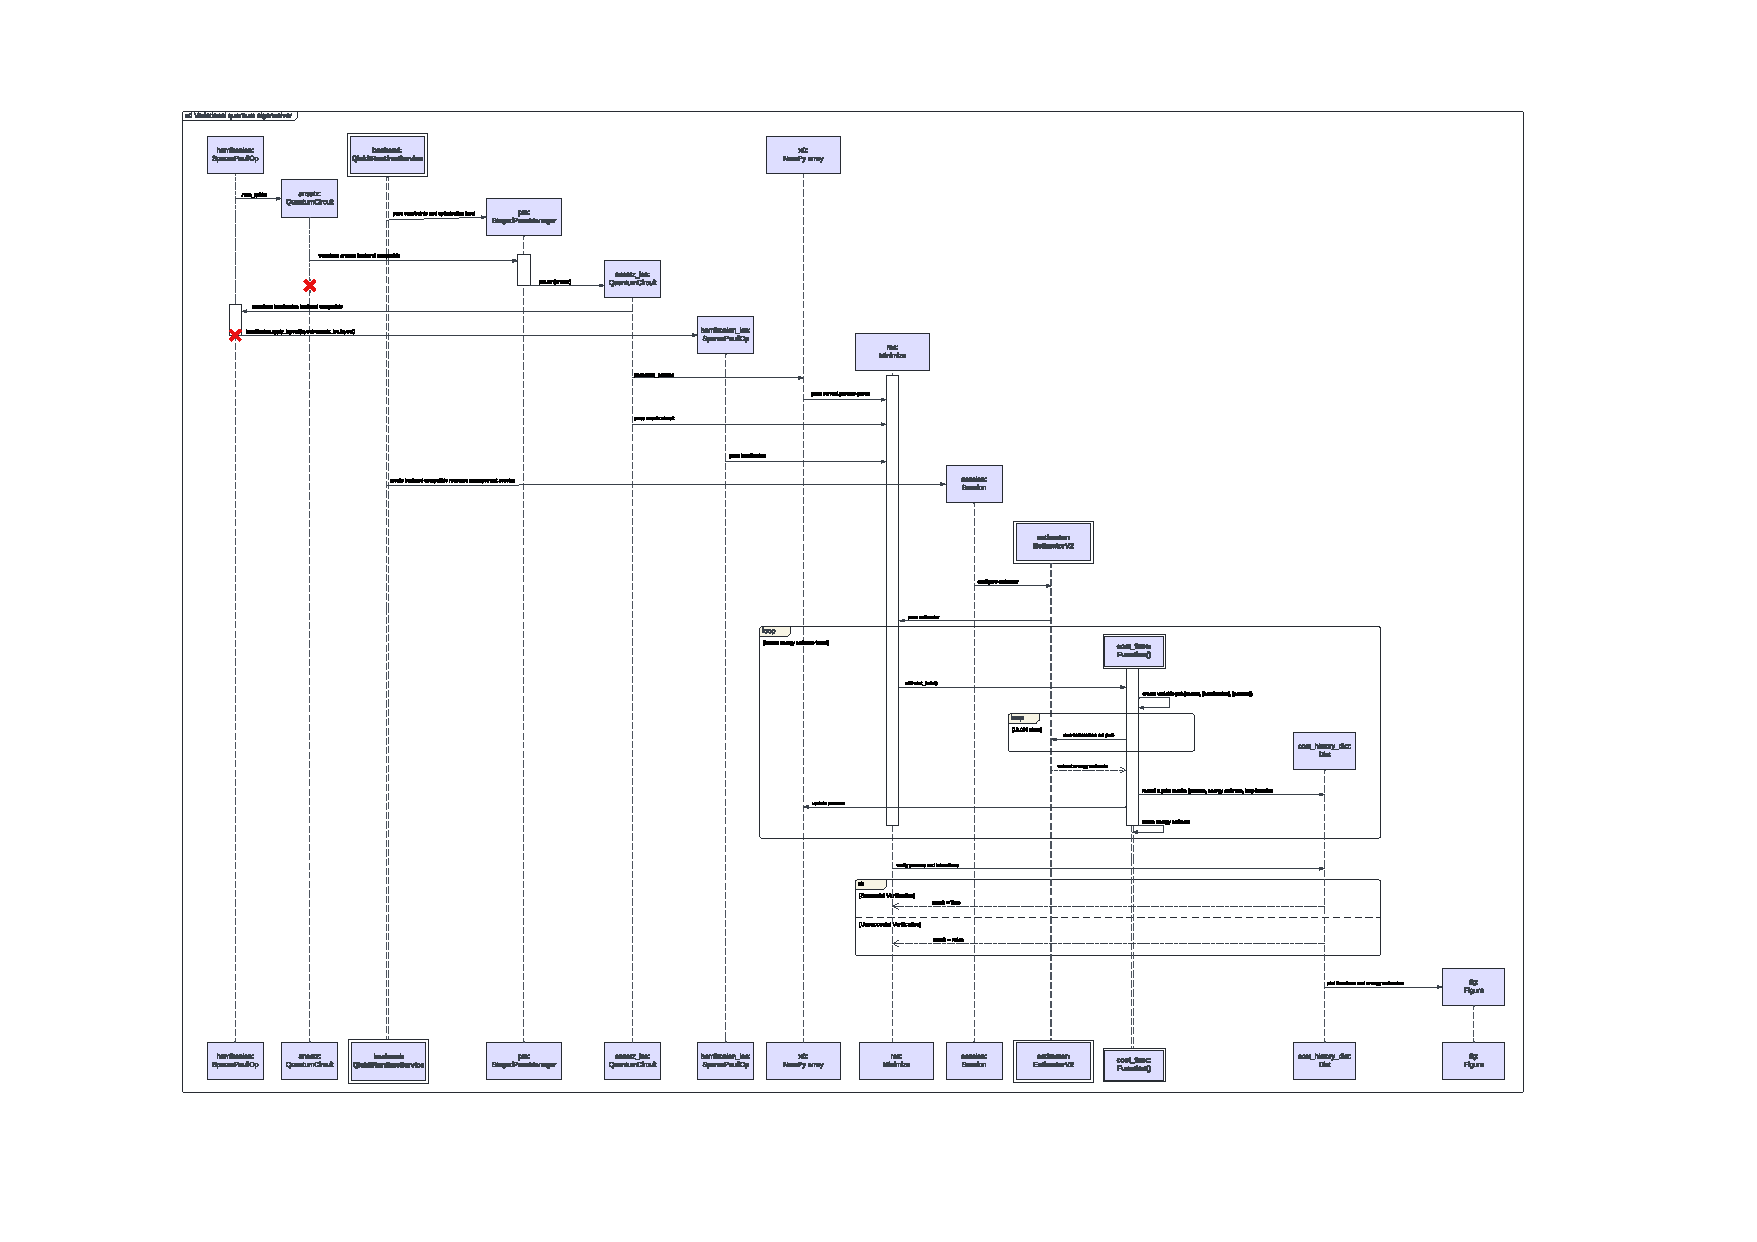
\includegraphics[width=1\linewidth]{VQE QUML SD Final Version.pdf}
    \caption{The application of Q-UML to a sequence diagram modelling the IBM Quantum Learning VQE Algorithm.}
    \label{fig:Q-UML_SD}
\end{sidewaysfigure}

\subsubsection{SD Quantum UML Profile}

The \textbf{backend} element, responsible for facilitating communication with quantum software, is assigned the stereotype \texttt{<<Quantum Driver>>}.

The \textbf{estimator} element, whose functionality executes quantum circuits, is assigned the stereotype \texttt{<<Quantum>>}.

The \textbf{cost\_func} element is directly tied to the interaction where a \texttt{<<Quantum Driver>>} invokes the \texttt{<<Quantum>>} element. It includes the operation \textit{estimator.run()} to execute this call, making it appropriate to assign the stereotype \texttt{<<Quantum Request>>}. The classical optimiser, \textbf{res}, is involved in this process but does not directly call \textit{estimator.run()}. Instead, it uses the classical output from \textbf{cost\_func} and provides classical input to the instance \textbf{x0}. As its interactions remain classical, \textbf{res} is not assigned a quantum stereotype.

Similarly to Q-UML, the message from \textbf{cost\_func} calling the estimator's \textit{.run()} method is assigned the \texttt{<<Quantum Request>>} stereotype as it is a message containing quantum information. There is no \texttt{<<Quantum Reply>>} stereotype as the estimator converts the message back into classical information before being received by \textbf{cost\_func}.

The corresponding diagram is presented in Figure 9.

\begin{sidewaysfigure}
    \centering
    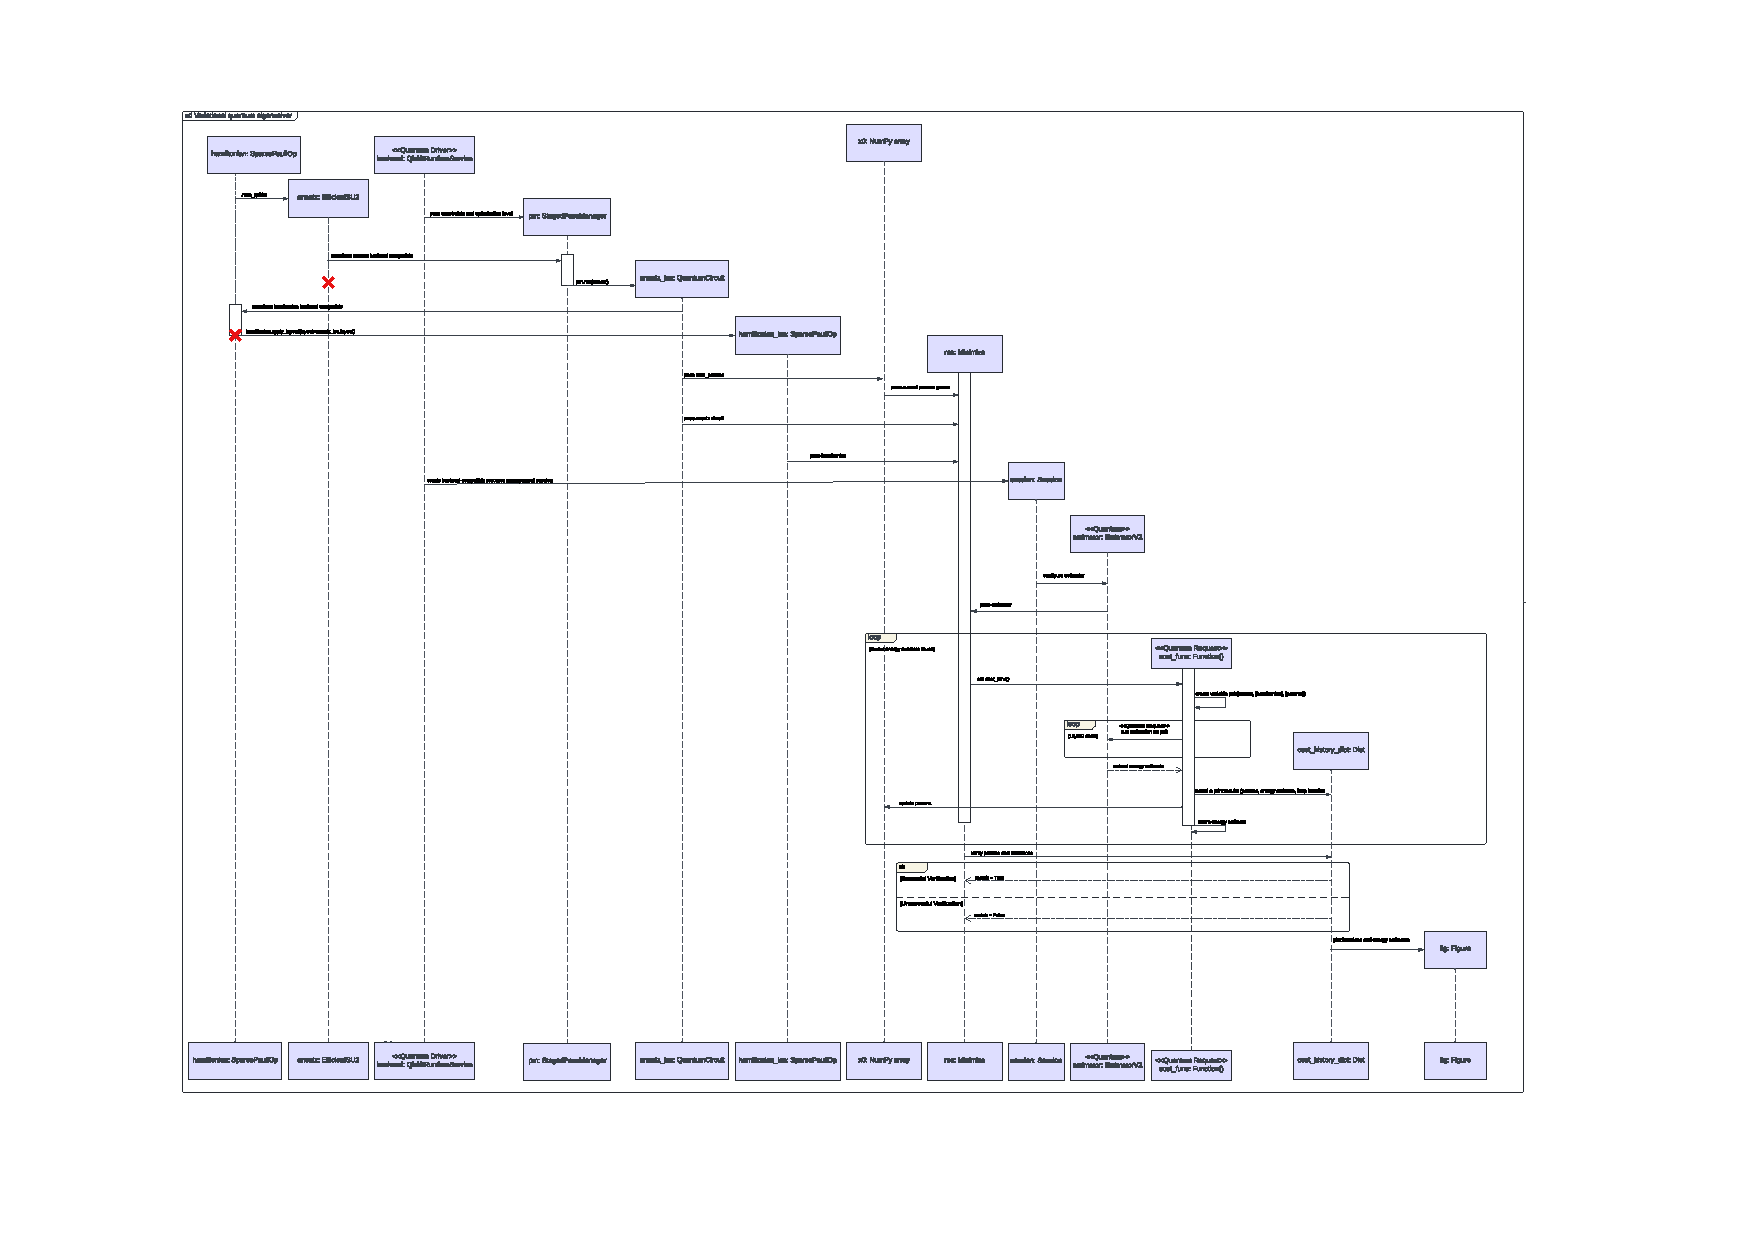
\includegraphics[width=1\linewidth]{VQE UML Profile SD Final Version.pdf}
    \caption{The application of the quantum UML profile to a sequence diagram modelling the IBM Quantum Learning VQE Algorithm.}
    \label{fig:QUMLP_SD}
\end{sidewaysfigure}

\subsection{VQE Class Diagram}

Packages group the Python libraries and Qiskit SDK imports needed to execute the VQE algorithm, providing a clear visual of the required dependencies. Packages consist of a boundary, similar to the frame, loop and alt fragments, with the package name appearing outside of the boundary in the upper-left corner. The package \textbf{NumPy} is embedded within the Qiskit package—a design choice to prevent overlapping edges rather than imply a nested structure.

The class diagram elements, depicted as rectangles, illustrate the classes used in the Qiskit VQE algorithm, with each rectangle divided into three sections: namespace, attributes, and operations. A design choice was made to keep the same notation of \textit{instance:Class} for the namespace. This notation is typically used in object diagrams and not for class diagrams. Class diagrams provide a static system view and usually only include the class name. In contrast, object diagrams capture the system at runtime and use either \textit{instance}, \textit{instance:Class} or \textit{:Class} as its naming convention\cite{Seidl_Scholz_Huemer_Kappel_Duffy_2014}. The decision to retain the instance in the notation is for clarity's sake, providing a minimal but effective indication of which class represents what aspect of the VQE algorithm by the instance name. Without an in-depth knowledge of Qiskit, it may be challenging to determine that \textbf{EfficentSU2} represents the ansatz or \textbf{SparsePauliOp} represents the Hamiltonian.

A separate diagram was created for the \textbf{Minimize} class, distinct from the \textbf{CostFunction} class. Attempts to depict all class connections in a single diagram led to overlapping edges and clutter. The resulting diagram remains clear and readable by isolating \textbf{Minimize} and connecting it with simplified classes representing its connections to the larger diagram. The simplified classes are enclosed within the Qiskit package to indicate the part of the system they belong to. Due to visual alignment issues, the class \textbf{CostFunction} is not contained in this package. Given the full context of the diagram, its role should still be evident. 

Only the attributes and methods relevant to the VQE algorithm are shown; additional attributes and methods documented in these classes have been omitted for clarity.

Some elements in the diagram, such as \textbf{Numpy.ndarray}, \textbf{CostFunction}, and \textbf{Dict}, are user-defined classes and therefore lack documentation detailing their attributes and operations. The variables and methods within these objects are presented in the diagram as the attributes and operations of these elements.

Each class attribute and method contains a visibility marker and it's name with the format "visbility\textbf{name:}". The visibility of all attributes and methods within the system is public, distinguished by the character +, meaning they are accessible to all other objects within the system\cite{Seidl_Scholz_Huemer_Kappel_Duffy_2014}. This was determined by none of the attributes or methods containing a leading underscore, which is the convention used in Python to indicate a private attribute or method\cite{Privacy}.

Class attributes contain their data type with the format "visbility\textbf{name:} data type". Some class attributes also include multiplicities, which can be seen in the classes \textbf{SparsePauliOp}, \textbf{EfficientSU2}, \textbf{QiskitRuntimeService}, \textbf{EstimatorV2}, \textbf{Dict}, and \textbf{Pyplot}. Attribute multiplicities are used in these classes to convey how many values the attribute can hold, with [0...1] indicating either none or one value or [1...*] to indicate one or many values\cite{Seidl_Scholz_Huemer_Kappel_Duffy_2014}. Attributes, where multiplicities are omitted, are considered to have only one value\cite{Seidl_Scholz_Huemer_Kappel_Duffy_2014}. Attributes with multiplicities also have additional information as to whether the values can be duplicated with the terms "unique" or "non-unique" and whether the values must be in a fixed order with the terms "ordered" or "unordered"\cite{Seidl_Scholz_Huemer_Kappel_Duffy_2014}. The format for an attribute which contains all of these details is "visbility\textbf{name:} data type[multiplicity]\{duplication,order\}". When an attribute's data type is a tuple, such as the \textbf{pub} attribute in \textbf{CostFunction}, each item's name and data type are specified, with square brackets enclosing the tuple to indicate its structure. Attributes can have various data types. For instance, the \textbf{mode} attribute of \textbf{EstimatorV2} can take data types beyond \textbf{Session}. Specific data types in the code are named rather than general classes from the documentation. For example, the returned data type for \textbf{StagedPassManager}'s \textit{.run()} method is \textbf{\_CircuitsT}, not \textbf{EfficientSU2}\cite{StagedPassManager}. Including attributes is optional, with some classes not requiring this information, such as \textbf{StagedPassManager} and \textbf{Session}. 

Class methods are shown with either empty parentheses if no parameter information is needed or with detailed parameter information listed within the parentheses. The data type of the returned value is provided after the parentheses. The typical notation for a method with parameter information is "visbility\textbf{name}(\textbf{parameter name:} parameter data type): returned data type. For methods returning tuples—such as the \textit{from\_list()} method in \textbf{SparsePauliOp}, the \textit{run()} method in \textbf{Estimator}, and the \textit{res()} method in \textbf{Minimize}—each item's name and data type are specified and enclosed in square brackets, mirroring the method's format in code. 
The methods \textit{set\_xlabel()} and \textit{set\_ylabel()} in the \textbf{Pyplot} class do not have a return data type, as they do not return a value\cite{xlabel}\cite{ylabel}. Instead, they update a Figure object by assigning relevant information. The final output of type Figure is produced when the \textit{draw()} method is executed. 
Some classes, like \textbf{CostFunction} and \textbf{Minimize}, are methods themselves. These classes include methods with the class instance name, indicating that the class can be executed as an operation. Including operations is optional, with some classes not requiring this information, such as \textbf{IBMBackend} and \textbf{Dict}. 

Associations between classes are depicted by the edges that join the rectangles of the diagram. Edges with a solid line and filled triangular arrowhead pointing from one class to another indicate a binary association, where one class can view the visible attributes and operations of another class, but not the other way round\cite{Seidl_Scholz_Huemer_Kappel_Duffy_2014}. For example, \textbf{Session} can view the attributes and operations of \textbf{QiskitRuntimeService}, but \textbf{QiskitRuntimeService} cannot view the attributes and operations of \textbf{Session}. The edges between \textbf{SparsePauliOp} and \textbf{EfficentSU2} do not have arrowheads, meaning they are bidirectional; each class can view the other's attributes and operations\cite{Seidl_Scholz_Huemer_Kappel_Duffy_2014}. As we established earlier, all attributes and operations in the system are public and can technically be accessed by all objects. In the context of this VQE implementation, the associations indicate which objects share and which objects receive information. Specifically, \textbf{SparsePauliOp} and \textbf{EfficientSU2} provide each other with information throughout the VQE algorithm. In contrast, \textbf{QiskitRuntimeService} provides information to \textbf{Session}, but \textbf{Session} does not provide information to \textbf{QiskitRuntimeService}.

The \textbf{IBMBackend} class depends on the \textbf{QiskitRuntimeService} class. This is depicted by a dashed line with an open arrowhead pointing from the dependent object to the object it depends on. The Qiskit documentation states that IBMBackend must not be instantiated directly and instead should be interacted with using the methods in \textbf{QiskitRuntimeService}\cite{IBMBackend}. The \textbf{IBMBackend} class is included in this diagram as its documentation contains the \textbf{target} attribute, which must be passed to \textbf{StagedPassManager} to access information regarding the selected quantum hardware constraints. The relationship has the stereotype \texttt{<<instantiate>>} as \textbf{IBMBackend} requires \textbf{QiskitRuntimeService} for it's full implementation\cite{Dependencyrelationships}.

The class \textbf{Dict} is a composition of the class \textbf{CostFunction}. A composition is a binary association signifying that one class is contained as part of another class and cannot exist without it; if the aggregate(whole) object is destroyed, the contained part is also destroyed\cite{Seidl_Scholz_Huemer_Kappel_Duffy_2014}. The relationship is depicted on the association edge by a filled diamond attached to the aggregate class. In this case, \textbf{Dict} is an integral part of \textbf{CostFunction} as it's contained within it. If \textbf{CostFunction} were destroyed, \textbf{Dict} would also be destroyed.

Shared aggregation is similar to composition in that it signifies that one class belongs to another. However, unlike a composition, the contained classes can exist outside the aggregated class\cite{Seidl_Scholz_Huemer_Kappel_Duffy_2014}. A hollow diamond attached to the aggregate class depicts the relationship on the association edge. Shared aggregation is used to describe classes that are passed as parameters to other classes in the VQE algorithm; \textbf{Numpy:ndarray}, \textbf{EfficentSU2}, \textbf{EstimatorV2}, and \textbf{SparsePauliOp} are all passed as parameters to \textbf{CostFunction} and therefore have shared aggregation. These classes, along with \textbf{CostFunction}, are passed to \textbf{Minimize}.

Some associations may be given an association name with a reading direction indicated by a filled triangular arrowhead pointing from one class to another. This arrowhead signifies the flow of the association's action, helping to clarify the direction in which information or control is passed between the classes involved\cite{Seidl_Scholz_Huemer_Kappel_Duffy_2014}. For example, the association between \textbf{StagedPassManager} and \textbf{EfficientSU2} shows that the pass manager will transform the ansatz and not the other way around. Although the reading direction points in the same direction as the binary association in this example, it does not have to\cite{Seidl_Scholz_Huemer_Kappel_Duffy_2014}.

Associations between classes contain multiplicities, which specify how many objects are involved in each association. For instance, the binary association between \textbf{StagedPassManager} and \textbf{EfficientSU2} demonstrates that one instance of \textbf{StagedPassManager} is associated with exactly one instance of \textbf{EfficientSU2}. Multiplicities in the diagram are either 1 or 1..*, with the option to label shared attributes. In the case of the \textbf{Minimize} class, it shares between one and many values of the attribute \textbf{res.x}—which contains parameters it iteratively updates—with a single \textbf{Numpy.ndarray} object. 
Subsequently, \textbf{Numpy.ndarray} shares a single array object with \textbf{CostFunction}, with only its values being updated. The use of multiplicities conveys a single-instance relationship between \textbf{Numpy.ndarray} and \textbf{CostFunction} while showing that \textbf{Minimize} dynamically updates and shares multiple values of \textbf{res.x} to the \textbf{Numpy.ndarray} class.

\subsubsection{CD QUML}

The classes \textbf{CostFunction}, \textbf{QiskitRuntimeService}, \textbf{IBMBackend}, and \textbf{EstimatorV2} are depicted as quantum. This remains consistent with the sequence diagram quantum object labelling, with the inclusion of \textbf{IBMBackend} being a dependent object of \textbf{QiskitRuntimeService}.

No quantum attributes are shown, as all quantum data is translated into classical information for storage within these classes.

Quantum operations, input, and output data types are written in bold to indicate their quantum nature. The \textbf{QiskitRuntimeService} class includes two operations that return the class \textbf{IBMBackend} as a quantum data type. The sole operation of the \textbf{Session} class also outputs an \textbf{IBMBackend} quantum data type. The \textbf{EstimatorV2} class features a quantum operation, \textit{.run()}, which interacts with quantum hardware and returns an object of the class \textbf{RuntimeJobV2}. While the returned information remains classical, \textbf{RuntimeJobV2} is intrinsically tied to a quantum communication process of extracting and translating quantum information as a classical output. Consequently, \textbf{RuntimeJobV2} is classified as a quantum data type.

The \textbf{CostFunction} class contains itself as the quantum operation \textit{cost\_func()}, which accesses quantum information when called and returns a classical data type. The \textbf{Minimize} class contains the \textit{res()} operation, which accepts \textbf{CostFunction} and a tuple as its parameters, requiring the quantum input data types \textbf{EstimatorV2} and \textbf{CostFunction}.

A single quantum aggregation relationship exists between \textbf{EstimatorV2} and \textbf{CostFunction}, represented by a double-lined edge. In this relationship, the \textbf{EstimatorV2} quantum class is passed as a parameter to the \textbf{CostFunction} quantum class.

The corresponding diagram is presented in Figure 10.

\begin{sidewaysfigure}
    \centering
    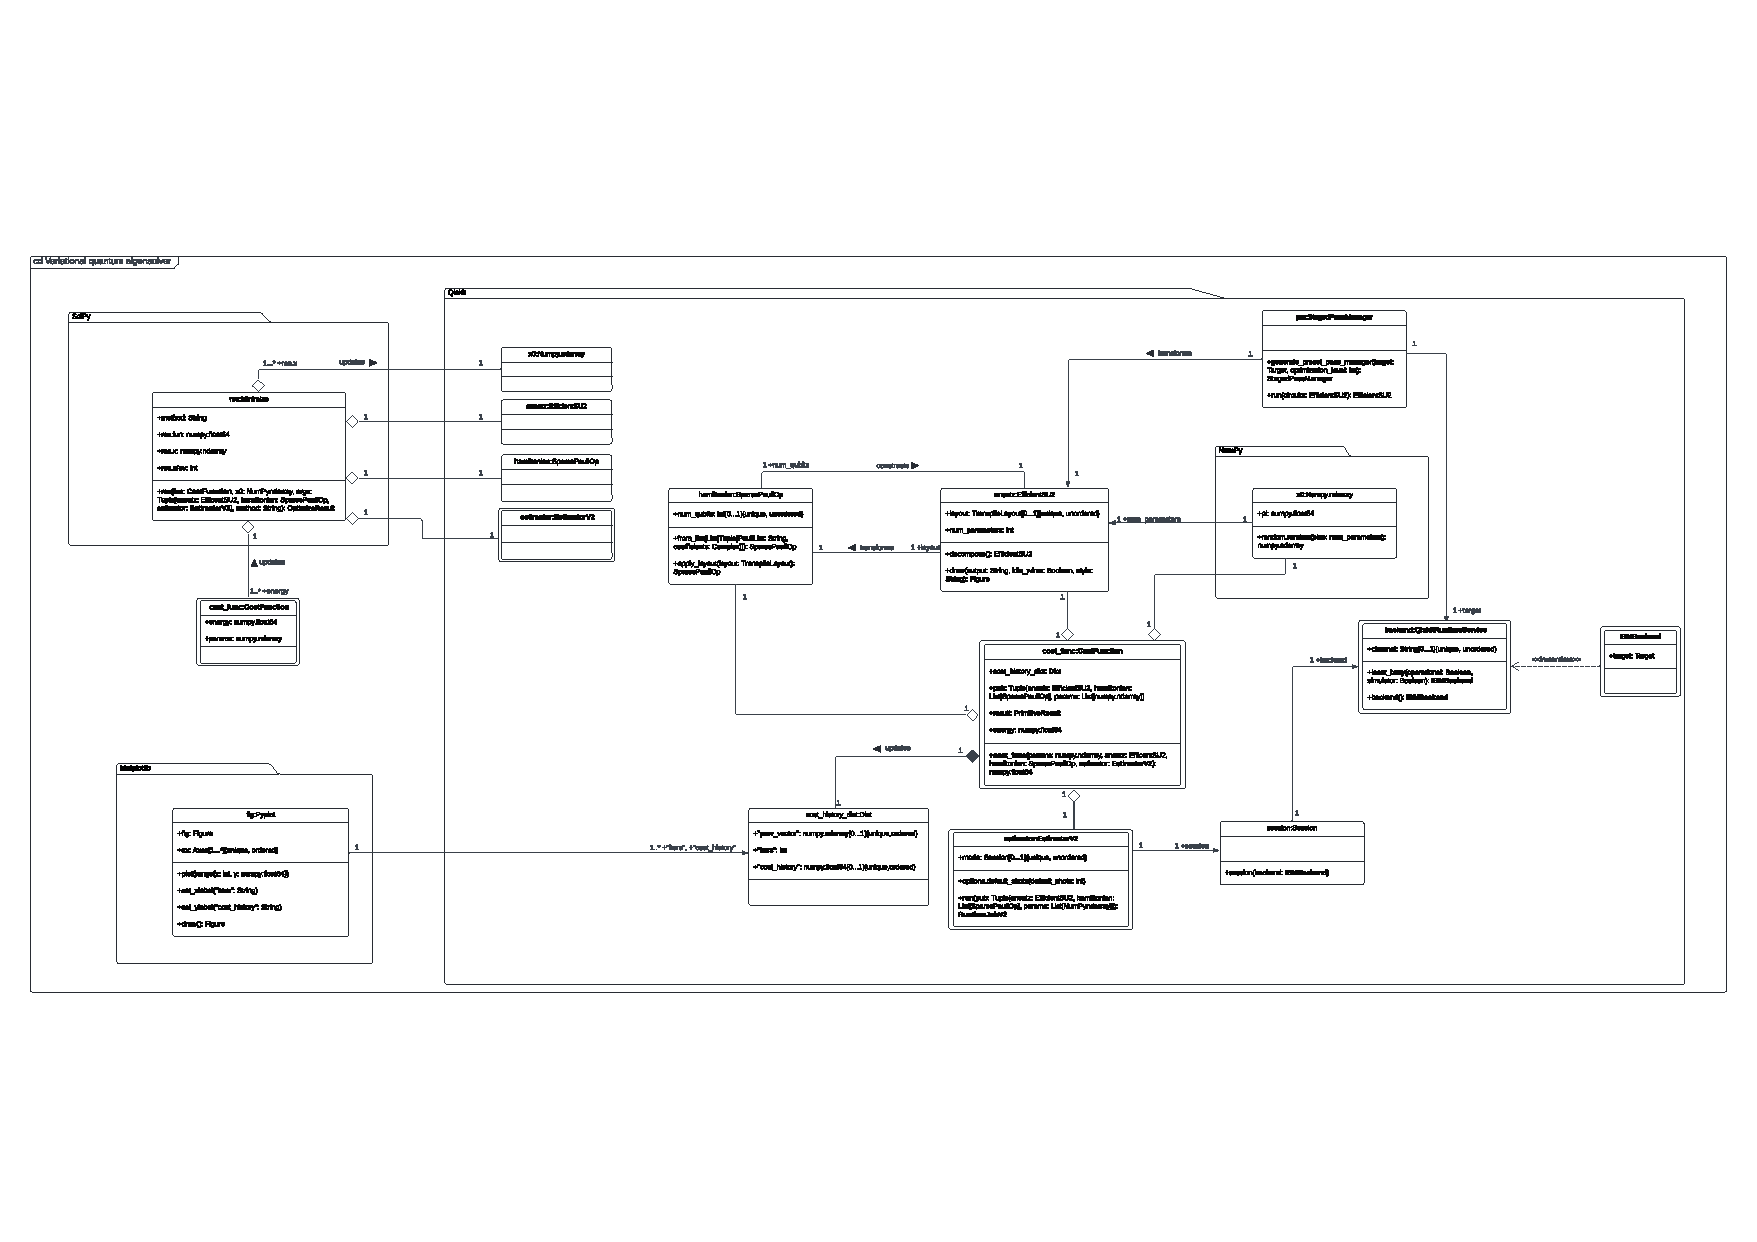
\includegraphics[width=1\linewidth]{VQE QUML CD Final Version.pdf}
    \caption{The application of Q-UML to a class diagram modelling the IBM Quantum Learning VQE Algorithm.}
    \label{fig:Q-UML_CD}
\end{sidewaysfigure}

\subsubsection{CD Quantum UML Profile}

The Qiskit package is assigned the stereotype \texttt{<<Quantum>} as it is a package that enables quantum functionality, allowing users to access quantum computers through the Qiskit SDK. 

The classes \textbf{CostFunction}, \textbf{EstimatorV2}, and \textbf{QiskitRuntimeService} inherit the same stereotypes as those assigned to their counterpart lifelines in the sequence diagram. Additionally, the \textbf{IBMBackend} class, which depends on \textbf{QiskitRuntimeService}, is also assigned the \texttt{<<Quantum Driver>>} stereotype.

The operation \textit{.run()} in \textbf{EstimatorV2} and \textit{cost\_func()} in \textbf{CostFunction} are assigned the stereotype \texttt{<<Quantum Request>>}. Both operations are quantum as discussed previously; \textit{estimator.run()} invokes a call from the \texttt{<<Quantum Driver>>} to the \texttt{<<Quantum>>} estimator and \textbf{CostFunction} contains this operation in it's design.

The corresponding diagram is presented in Figure 11.

\begin{sidewaysfigure}
    \centering
    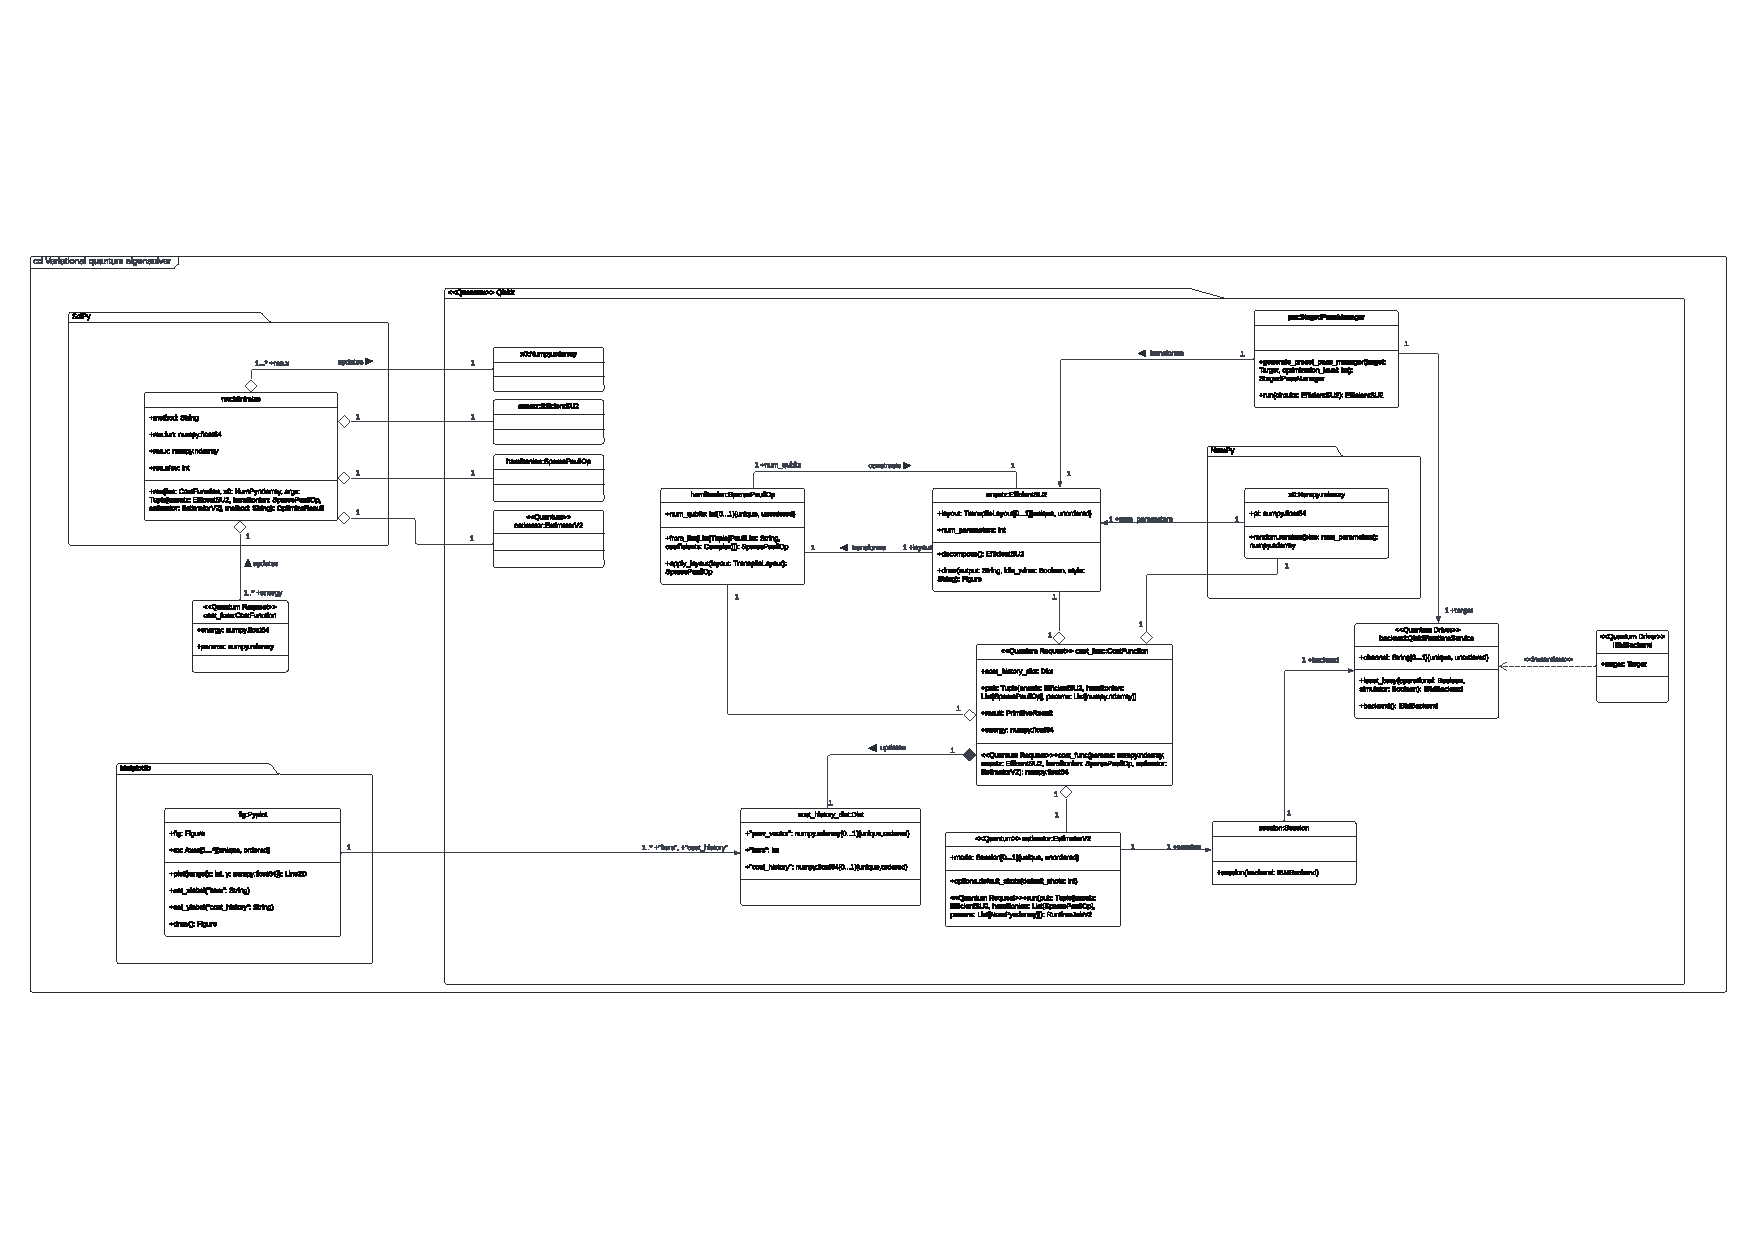
\includegraphics[width=1\linewidth]{VQE UML Profile CD Final Version.pdf}
    \caption{The application of the quantum UML profile to a class diagram modelling the IBM Quantum Learning VQE Algorithm.}
    \label{fig:QUMLP_CD}
\end{sidewaysfigure}

\section{Results and Analysis}

This section will discuss the results of analysing the two quantum UML adaptations. It begins with the author's thoughts on several aspects: analysing each diagram's construction, visibility, conveyed information, and the challenges encountered during their creation. It then assesses each diagram using five established characteristics for effective software modelling. 

\subsection{Author's Analysis}

\subsubsection{Diagram Construction}

A combination of PlantUML and Lucidchart was required to create the Q-UML versions of the UML diagrams. While efforts were made to incorporate double-lined notation using PlantUML, a Q-UML extension for PlantUML would be necessary to create diagrams using the complete Q-UML notation.

PlantUML proved significantly easier to use for sequence diagrams compared to Lucidchart, which required extensive manual adjustments that were both cumbersome and time-consuming. The quantum UML profile for sequence diagrams could have been created entirely in PlantUML, as its notation is fully UML-compliant and supported by built-in extensions, simplifying the process.

This was not the case for class diagrams. Attempts to construct them using PlantUML and Mermaid, another open-source text-based diagramming tool, produced messy and convoluted results, making direct translation into Lucidchart impractical. Design adjustments were necessary, such as isolating the \textbf{Minimize} class into a stand-alone diagram and linking it to the central diagram. While this may have been achievable in either PlantUML or Mermaid, it was unclear how to do so immediately. For simplicity and due to time constraints, the class diagrams were constructed solely in Lucidchart. Insights gathered during the research and development phase highlighted PlantUML's limitations in managing the scope of larger projects\cite{plantreddit}. The diagrams created in PlantUML and Mermaid are given in the appendix. 

\subsubsection{Diagram Visibility}

When observing the diagrams in full, Q-UML stands out for its clear indication of quantum elements. Double lines highlighting quantum components allow for clear distinction when viewing the diagrams at a distance. The bold font used for names, data types and messages is less prominent. The quantum UML profile adaptations require closer inspection to discern any of its quantum details.

The diagrams are notably large, representing a relatively small code example, which reduces the visibility of the content when the diagrams are observed in full. While the sequence diagram closely follows the output of PlantUML and might have adopted a different scale if drawn manually, the class diagrams were manually constructed. Whether the size of these diagrams poses a concern is open to debate. They accurately depict the exact implementation of the VQE algorithm as outlined in IBM's tutorial, raising a fundamental question: should UML have been used to document a specific code implementation, or would it have been more appropriate to model the general steps required to implement VQE in Qiskit? This distinction could significantly affect the design and scale of the diagrams.

UML is a versatile modelling language suited for designing new systems and analysing existing ones. While using UML to model exact code implementations is valid, it restricts comparisons with other examples. The Q-UML and quantum UML profile papers are the only known works that implement UML diagrams in a quantum context. Like this paper, Q-UML uses Lucidchart, allowing for fairer evaluation, but models Shor's algorithm—a fundamentally different case—rather than a specific code implementation. In contrast, the quantum UML profile examples depict a general hybrid algorithm in a broader system, including a class diagram of a financial web application\cite{Pérez-Castillo2022}. These examples succinctly model larger systems, whereas this paper struggled with a relatively small amount of code. The quantum UML profile diagrams were created using Papyrus, a bespoke UML modelling tool which may better handle scalability. The use of different modelling tools makes direct comparisons challenging.

To fully evaluate the suitability of the created diagrams, they would need to be compared to similar ones—specifically, UML diagrams depicting the implementation of hybrid algorithms in a modern programming language. Given more time, revisions could include exploring alternative diagram versions, focusing on different implementations of VQE, modelling the algorithm rather than its specific realisation in Qiskit, or alternative hybrid algorithms implemented in code. Producing additional diagrams would enhance the design quality through iterative practice and provide a broader body of work for cross-comparison.

Despite these limitations, the scale of the diagrams may not be a significant issue, as their details remain readily accessible upon closer examination.

\subsubsection{Diagram Information}

In the context of this paper's UML diagrams, the quantum UML profile offers more nuanced insights into quantum elements and messages compared to Q-UML. It explicitly distinguishes between quantum components, components facilitating quantum communication and components involved in requests to quantum hardware. Conversely, Q-UML uses the same pictorial notation for all these element types, limiting the information about each element's specific role.

Despite this, Q-UML excels in representing quantum data types. The quantum UML profile’s use of stereotype tags for data types can appear visually cluttered, making them less distinguishable than Q-UML’s approach. The stereotype tags are also restricted to predefined categories, limiting their applicability to all quantum data types within a class. In contrast, Q-UML's use of bold font and a more flexible approach to quantum labelling enables visually clearer and more detailed modelling of quantum data types within classes.

A hybrid approach, combining the quantum UML profile with Q-UML's use of bold text for quantum data types, could present a promising alternative.

\subsubsection{Challenges}

Determining which data types and classes to classify as quantum was a key challenge in creating the UML diagrams. Identifying quantum elements required a thorough analysis of Qiskit’s documentation, focusing on the roles and interactions of each class or data type within the operation. Ultimately, only those classes known to be involved in interactions with IBM's quantum computers could be definitively classified as quantum. 

When applying the Q-UML notation, challenges arose in determining whether the class \textbf{Minimize} should be classified as quantum. Since it accepts quantum elements as parameters, it was considered a candidate for quantum classification under the principles of quantum supremacy or quantum aggregation. According to the quantum supremacy principle, an element should be classified as quantum \textit{"if and only if it contains quantum elements"}\cite{Pérez-Castillo2022}. While \textbf{Minimize} accepts the quantum elements \textbf{CostFunction} and \textbf{EstimatorV2} as parameters, it does not \underline{contain} their quantum information. Instead, it retrieves the classical output from \textbf{CostFunction} and passes \textbf{EstimatorV2} to \textbf{CostFunction} without directly handling quantum data, as any quantum information is transformed into classical form before \textbf{Minimize} interacts with it.

Similarly, quantum aggregation does not apply, even though shared aggregation is used to represent parameter-passing relationships in the diagram. The \textbf{Minimize} class is not composed of the quantum elements it receives as parameters; its operation interacts exclusively with the classical output of \textbf{CostFunction} and communicates on a classical channel with \textbf{Numpy.ndarray} to update the parameters.

This raises an important question: what is the purpose of distinguishing quantum elements in UML? The need to differentiate between quantum and classical information has already been discussed earlier in the paper, with these different types of information holding fundamentally different characteristics which are not interchangeable. However, when using an SDK like Qiskit, quantum computations are performed externally, and any quantum information is translated back into classical data before being presented to the user. As a result, from the user’s perspective, all data types appear classical. 

This highlights another limitation of UML diagrams closely tied to specific code samples. An alternative UML diagram for VQE, independent of any programming language, could provide a clearer perspective on identifying quantum classes. However, determining data types might remain challenging without the context provided by a programming language.

Another approach to addressing this question could involve applying UML on a larger scale. For example, a UML diagram illustrating the structure of the Qiskit Runtime Service could provide deeper insights into defining classical and quantum elements within the Qiskit SDK and contextualise their roles within the broader system architecture. 

Distinguishing between classical and quantum elements is particularly valuable for cost analysis. Given the significantly higher expense of quantum hardware and information processing, identifying which system components rely on quantum resources provides essential insights into operational costs. The diagrams in this paper focus on a small code example with minimal quantum hardware access, limiting their effectiveness for comprehensive cost evaluation. A broader system model integrating classical and quantum hardware would offer a more complete perspective. A promising approach could involve modelling the VQE algorithm in Qiskit on a larger scale, incorporating its interactions with the Qiskit Runtime Service. This approach would present a diagram similar in design to the class diagram of the financial application in the quantum UML profile\cite{Pérez-Castillo2022}. This would be an excellent opportunity for direct diagram comparison, though it should ideally involve using the same modelling tool, Papyrus.

\subsection{Model Quality}

To evaluate the quality of each quantum UML adaptation, we will compare each model against Bran Selic's five characteristics for effective and useful modelling, as outlined in his 2003 paper, \textit{"The Pragmatics of Model-Driven Development,"} which highlights the advantages of model-driven development(MDD) in software engineering\cite{1231146}.

The five characteristics are: \textit{abstraction}, \textit{understandability}, \textit{accuracy}, \textit{predictiveness}, and \textit{cost-effectiveness}. A model should \textit{abstract} away from the system it represents, hiding irrelevant details to avoid over-complication. It must possess \textit{understandability}, ensuring the information it conveys is intuitive and natural to users. This includes expressivity, allowing complex information to be presented simply, requiring minimal domain-specific knowledge for comprehension. The model must ensure \textit{accuracy} by correctly representing the real-world system it is modelling. A model should also exhibit \textit{predictiveness}, enabling the discovery of interesting but non-obvious behaviours of the system. Finally, it should demonstrate \textit{cost-effectiveness}, ensuring it is cheaper to create the model than to build the actual system\cite{1231146}.

\subsubsection{Abstraction}

Q-UML exhibits greater abstraction than the quantum UML profile, focusing on distinguishing quantum and classical information in a system using simple pictorial and textual notations. In contrast, the quantum UML profile provides more explicit details through stereotype tags, prioritising detailed differentiation over abstraction.

\subsubsection{Understandability}

Q-UML's notation is more understandable than the quantum UML profile's. Its simple pictorial and textual notations clearly distinguish quantum and classical components, requiring no prior knowledge of what defines a quantum component. While the quantum UML profile necessitates familiarity with the paper's profile diagrams and the associated stereotype tags to interpret the different quantum elements, the distinction between quantum and classical remains clear, as quantum elements contain stereotype tags while classical elements do not.

\subsubsection{Accuracy}

Both adaptations accurately model the system by distinguishing its quantum and classical elements. The quantum UML profile offers greater specificity in categorising quantum components, which may make it more suitable for Model-Driven Development (MDD) applications. In MDD, models are not used just as a means of documentation but serve as the foundation for creating software, bypassing the need for traditional programming languages\cite{LUCIO2014103}. By providing detailed functionality for model elements rather than generic quantum labelling, the quantum UML profile could support the development of a low-code language, enabling the execution of algorithms like VQE directly from a model.

\subsubsection{Predictiveness}

This characteristic is difficult to evaluate. Since the diagrams explicitly represent an existing code implementation, there is little to no opportunity to implement the models themselves into code for testing. To accurately assess this, it would be necessary to create quantum UML models for a system that has not yet been coded and then generate code based on the models' depictions. This approach would allow for experimentation and validation of their effectiveness.

\subsubsection{Cost-effectiveness}

The quantum UML profile and the code excerpt it models are freely accessible. IBM provides 10 minutes of free monthly access to their quantum resources, and the diagrams can be created using free tools such as PlantUML, Papyrus, and Mermaid. In contrast, creating a Q-UML-compliant model required a paid Lucidchart subscription, making it more expensive than the system. If a Q-UML extension were developed for one of the available open-source UML tools, its associated cost could be eliminated.

\section{Conclusions}

This paper aimed to determine which quantum UML adaptation offers the best solution. Analysis revealed that both contain strengths and weaknesses: the quantum UML profile provides greater specificity, while Q-UML offers more flexibility. The choice ultimately depends on the user's purpose and audience—whether more detail benefits Q-SE professionals familiar with the domain or a more straightforward distinction between quantum and classical elements would suffice. The question of which model is "best" may be flawed, as both have merits and the available body of work for comparison is limited. This paper presents a small exploration of this topic; future comparisons of quantum UML methods to additional quantum algorithms or technologies could yield further insights. 

Comparing these diagrams with alternative quantum modelling approaches beyond UML would also offer a more comprehensive analysis. Other quantum modelling techniques have been explored and would have been valuable to consider against quantum UML adaptations if given more time\cite{9233151}\cite{app132111794}. This would also aid us in answering the question of whether a full-scale UML modelling should be adopted or a more simplified approach. Within the scope of this paper, Q-UML appears to be the more versatile choice for simpler modelling approaches, as its straightforward textual and graphical notation can extend beyond UML. In contrast, the quantum UML profile is inherently tied to UML's extension mechanism through profile diagrams. 

Some aspects of the Q-UML notation may require revision. Firstly, a minor issue in the example class diagram from the Q-UML paper shows multiplicities depicted using "m" rather than "*". Secondly, the UML standard for representing class names is to have them written in bold font\cite{Seidl_Scholz_Huemer_Kappel_Duffy_2014}. This presents a fundamental issue with Q-UML notation, which uses a bold font for all quantum elements. To address this, Q-UML may need to adopt an alternative notation for quantum elements, such as combining bold text with underlining or another distinguishing feature. The implementation of Q-UML notation for packages would also be beneficial. 

The quantum UML profile could benefit from more precise guidelines on when and how to apply its stereotypes. Currently, this information is primarily inferred from bullet-pointed explanations accompanying example diagrams. Adopting a methodology similar to Q-UML, which encapsulates such information within core design principles, could enhance usability for future researchers. Including notes or meta-attributes within the depicted meta-classes alongside the stereotypes could provide this clarity and aid in consistent implementation.

Regarding the objectives of the paper, the first objective was partially achieved. A real-world example of the VQE algorithm was chosen. However, the results showed that having an example bound to specific code implementation was counter-productive when trying to assess the suitability of the diagrams, particularly being able to answer the fourth modelling characteristic, predictiveness.

The second objective was successfully achieved. The sequence diagram was the most suitable model for illustrating the communication between elements required to execute VQE in Qiskit. Additionally, including the class diagram effectively complemented the sequence diagram by providing detailed insights into the elements' composition and the system's architecture.

The third objective was partially achieved but has room for improvement. Incorporating additional benchmarks for assessing modelling quality would strengthen the analysis, as the benchmark used, though relevant and cited, is over 20 years old and may not fully reflect current practices. Surveying software engineering and quantum computing professionals about quantum UML adaptations could enhance the methodology, particularly in evaluating whether UML remains an industry standard or if alternative modelling approaches are preferred. Insights during the research phase regarding UML's applicability to different industries were limited to informal discussions with a small group of peers and anecdotal insights from online forums\cite{redditumloften}. Expanding this inquiry to a broader, more diverse group could yield more definitive and actionable results. Despite these limitations, the analysis gave valuable insights into the strengths and weaknesses of the UML adaptations and offered several opportunities to extend this work in the future. 

The final objective was not achieved, as no additional diagrams or modelling of fundamental quantum properties were explored. Time constraints were a significant factor, compounded by the complexity of modelling quantum properties beyond the author’s current knowledge. This offers further work opportunities for those with a stronger understanding of quantum concepts.

The paper successfully summarises the contents of the two quantum UML adaptations, serving as a helpful reference for future researchers interested in applying these methods to their work. Additionally, it provides practical insights into UML modelling tools. Open-source options like PlantUML and Mermaid offer an accessible starting point for learning UML diagram construction but face challenges when scaling to larger systems. Lucidchart provides greater control and customisation, but its limitations include high costs (the free subscription was insufficient for this paper’s needs) and cumbersome manual adjustments when making edits. As demonstrated in the quantum UML profile literature, Papyrus may present a more suitable option for fully UML-compliant modelling, with its diagrams presented in the paper being in a concise, well-structured format.

While modelling a code-agnostic version of VQE may have been more beneficial for their comparisons, this paper highlights how much easier it is to convey information through diagrams than through a textual explanation. Comparing the diagrams to section 2.1.6.1, which aimed to provide context to the VQE Qiskit implementation, the diagrams are far more digestible. This highlights the necessity of modelling languages to communicate complex information effectively to professionals across diverse fields.

In conclusion, further exploration and development of quantum modelling techniques will enhance quantum modelling adaptations, build a robust comparative framework, and drive progress toward a universal quantum modelling language.

\section{Future Work}

Discussions on opportunities for future work have been highlighted throughout the Conclusion and the Results and Analysis sections. To summarise:

This work can be extended by applying the quantum UML adaptations to all fourteen UML diagram types. This paper and the foundational literature for these methods have explored only a limited subset.

Developing an extension for PlantUML or Mermaid to incorporate Q-UML notation would be a practical and valuable contribution to this research. This would not only improve accessibility but also serve as an excellent opportunity to merge theoretical work with a practical software development project. Lucidchart's beta feature, which supports importing Mermaid scripts for diagram creation, could provide a useful hybrid solution. This approach would allow users to construct diagrams using simple text notation and refine them within Lucidchart's GUI.

Another avenue for exploration is the applicability of the quantum UML profile in model-driven design. Investigating how quantum UML models could be adapted for building quantum software would deepen the practical relevance of these adaptations.

Finally, applying quantum UML adaptations and other quantum modelling techniques to diverse algorithms and broader systems—such as the Qiskit Runtime Service—could greatly enrich the field and drive the momentum Q-SE aims to achieve. There is ample opportunity to continue exploring alternative modelling tools, refining existing methodologies, establishing new benchmarks for model design, conducting broader comparisons, and engaging professionals across related industries. Sustained exploration and dialogue in this area are essential for achieving widespread adoption of Q-SE, particularly as quantum technologies progress toward significant developmental milestones.

\printbibliography

\section{Appendix}

\subsection{IBM Quantum Learning VQE Code}

Below is the example code provided by IBM Quantum Learning to implement the VQE algorithm in Qiskit\cite{Tutorial}.

\begin{lstlisting}[language=Python]
# General imports
import numpy as np

# Pre-defined ansatz circuit and operator class for Hamiltonian
from qiskit.circuit.library import EfficientSU2
from qiskit.quantum_info import SparsePauliOp

# SciPy minimizer routine
from scipy.optimize import minimize

# Plotting functions
import matplotlib.pyplot as plt

# Runtime imports
from qiskit_ibm_runtime import QiskitRuntimeService, Session
from qiskit_ibm_runtime import EstimatorV2 as Estimator

# To run on hardware, select the backend with the fewest number of jobs in the queue
service = QiskitRuntimeService(channel="ibm_quantum")
backend = service.least_busy(operational=True, simulator=False)

# Define Hamiltonian
hamiltonian = SparsePauliOp.from_list(
    [("YZ", 0.3980), ("ZI", -0.3980), ("ZZ", -0.0113), ("XX", 0.1810)]
)

# Create ansatz
ansatz = EfficientSU2(hamiltonian.num_qubits)
num_params = ansatz.num_parameters

# Initalise pass manager
from qiskit.transpiler.preset_passmanagers import generate_preset_pass_manager

target = backend.target
pm = generate_preset_pass_manager(target=target, optimization_level=3)

# Transform ansatz
ansatz_isa = pm.run(ansatz)

# Transform Hamiltonian
hamiltonian_isa = hamiltonian.apply_layout(layout=ansatz_isa.layout)

# Define Cost Function
def cost_func(params, ansatz, hamiltonian, estimator):
    """Return estimate of energy from estimator

    Parameters:
        params (ndarray): Array of ansatz parameters
        ansatz (QuantumCircuit): Parameterized ansatz circuit
        hamiltonian (SparsePauliOp): Operator representation of Hamiltonian
        estimator (EstimatorV2): Estimator primitive instance
        cost_history_dict: Dictionary for storing intermediate results

    Returns:
        float: Energy estimate
    """
    pub = (ansatz, [hamiltonian], [params])
    result = estimator.run(pubs=[pub]).result()
    energy = result[0].data.evs[0]

    cost_history_dict["iters"] += 1
    cost_history_dict["prev_vector"] = params
    cost_history_dict["cost_history"].append(energy)
    print(f"Iters. done: {cost_history_dict['iters']} [Current cost: {energy}]")

    return energy

# Initalise cost history dictionary
cost_history_dict = {
    "prev_vector": None,
    "iters": 0,
    "cost_history": [],
}

# Initalise parameters
x0 = 2 * np.pi * np.random.random(num_params)

# Run optimisation routine with COBYLA
with Session(backend=backend) as session:
    estimator = Estimator(mode=session)
    estimator.options.default_shots = 10000

    res = minimize(
        cost_func,
        x0,
        args=(ansatz_isa, hamiltonian_isa, estimator),
        method="cobyla",
    )

# Verify parameters
all(cost_history_dict["prev_vector"] == res.x)

# Verify iterations
cost_history_dict["iters"] == res.nfev

# Plot convergence
fig, ax = plt.subplots()
ax.plot(range(cost_history_dict["iters"]), cost_history_dict["cost_history"])
ax.set_xlabel("Iterations")
ax.set_ylabel("Cost")
plt.draw()

\end{lstlisting}

\subsection{PlantUML Diagrams}

Below are the class and sequence diagrams generated using PlantUML. The scripts for creating these diagrams are available in the GitHub repository associated with this paper\cite{ellygithub}.

\begin{figure}[H]
    \centering
    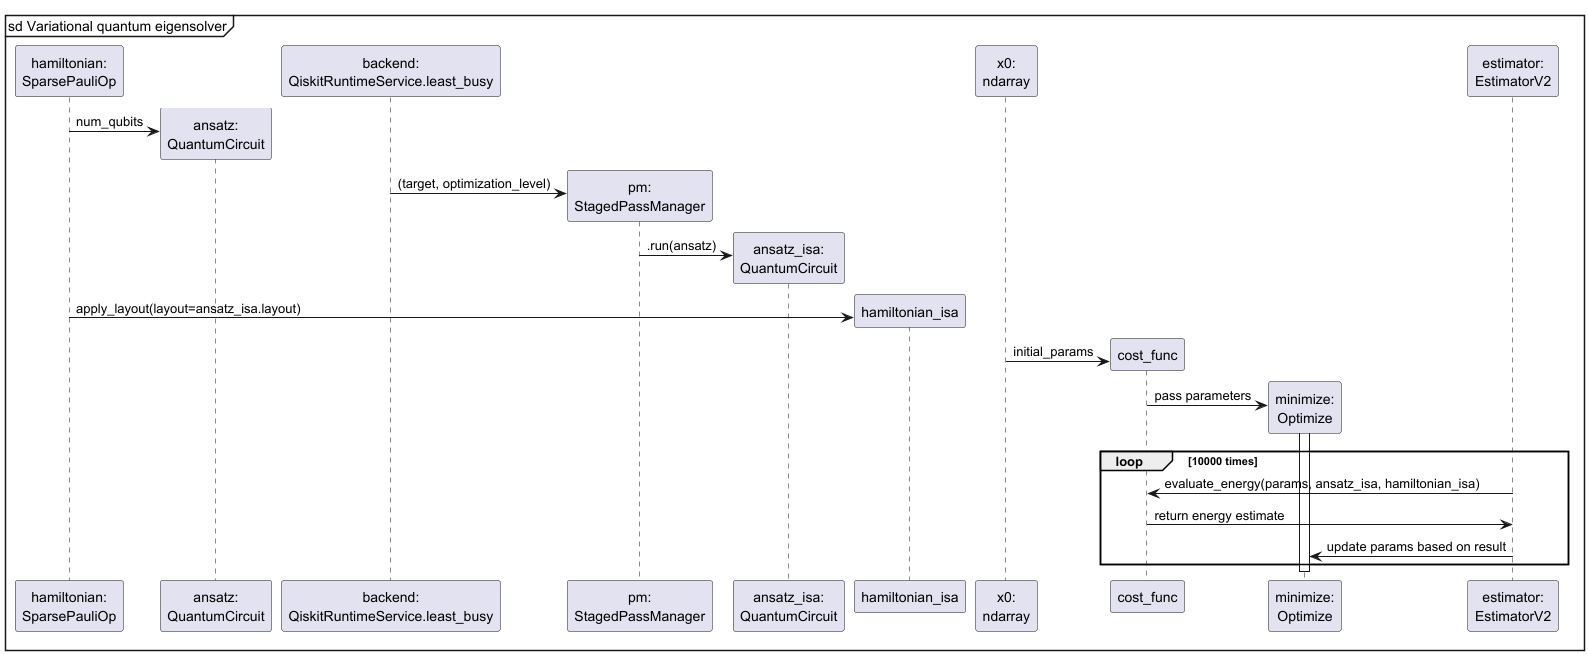
\includegraphics[width=1\linewidth]{vqe_sd_v1.png}
    \caption{First incomplete attempt at modelling VQE in a sequence diagram using PUML.}
    \label{fig:vqe_sd_v1}
\end{figure}

\begin{figure}[H]
    \centering
    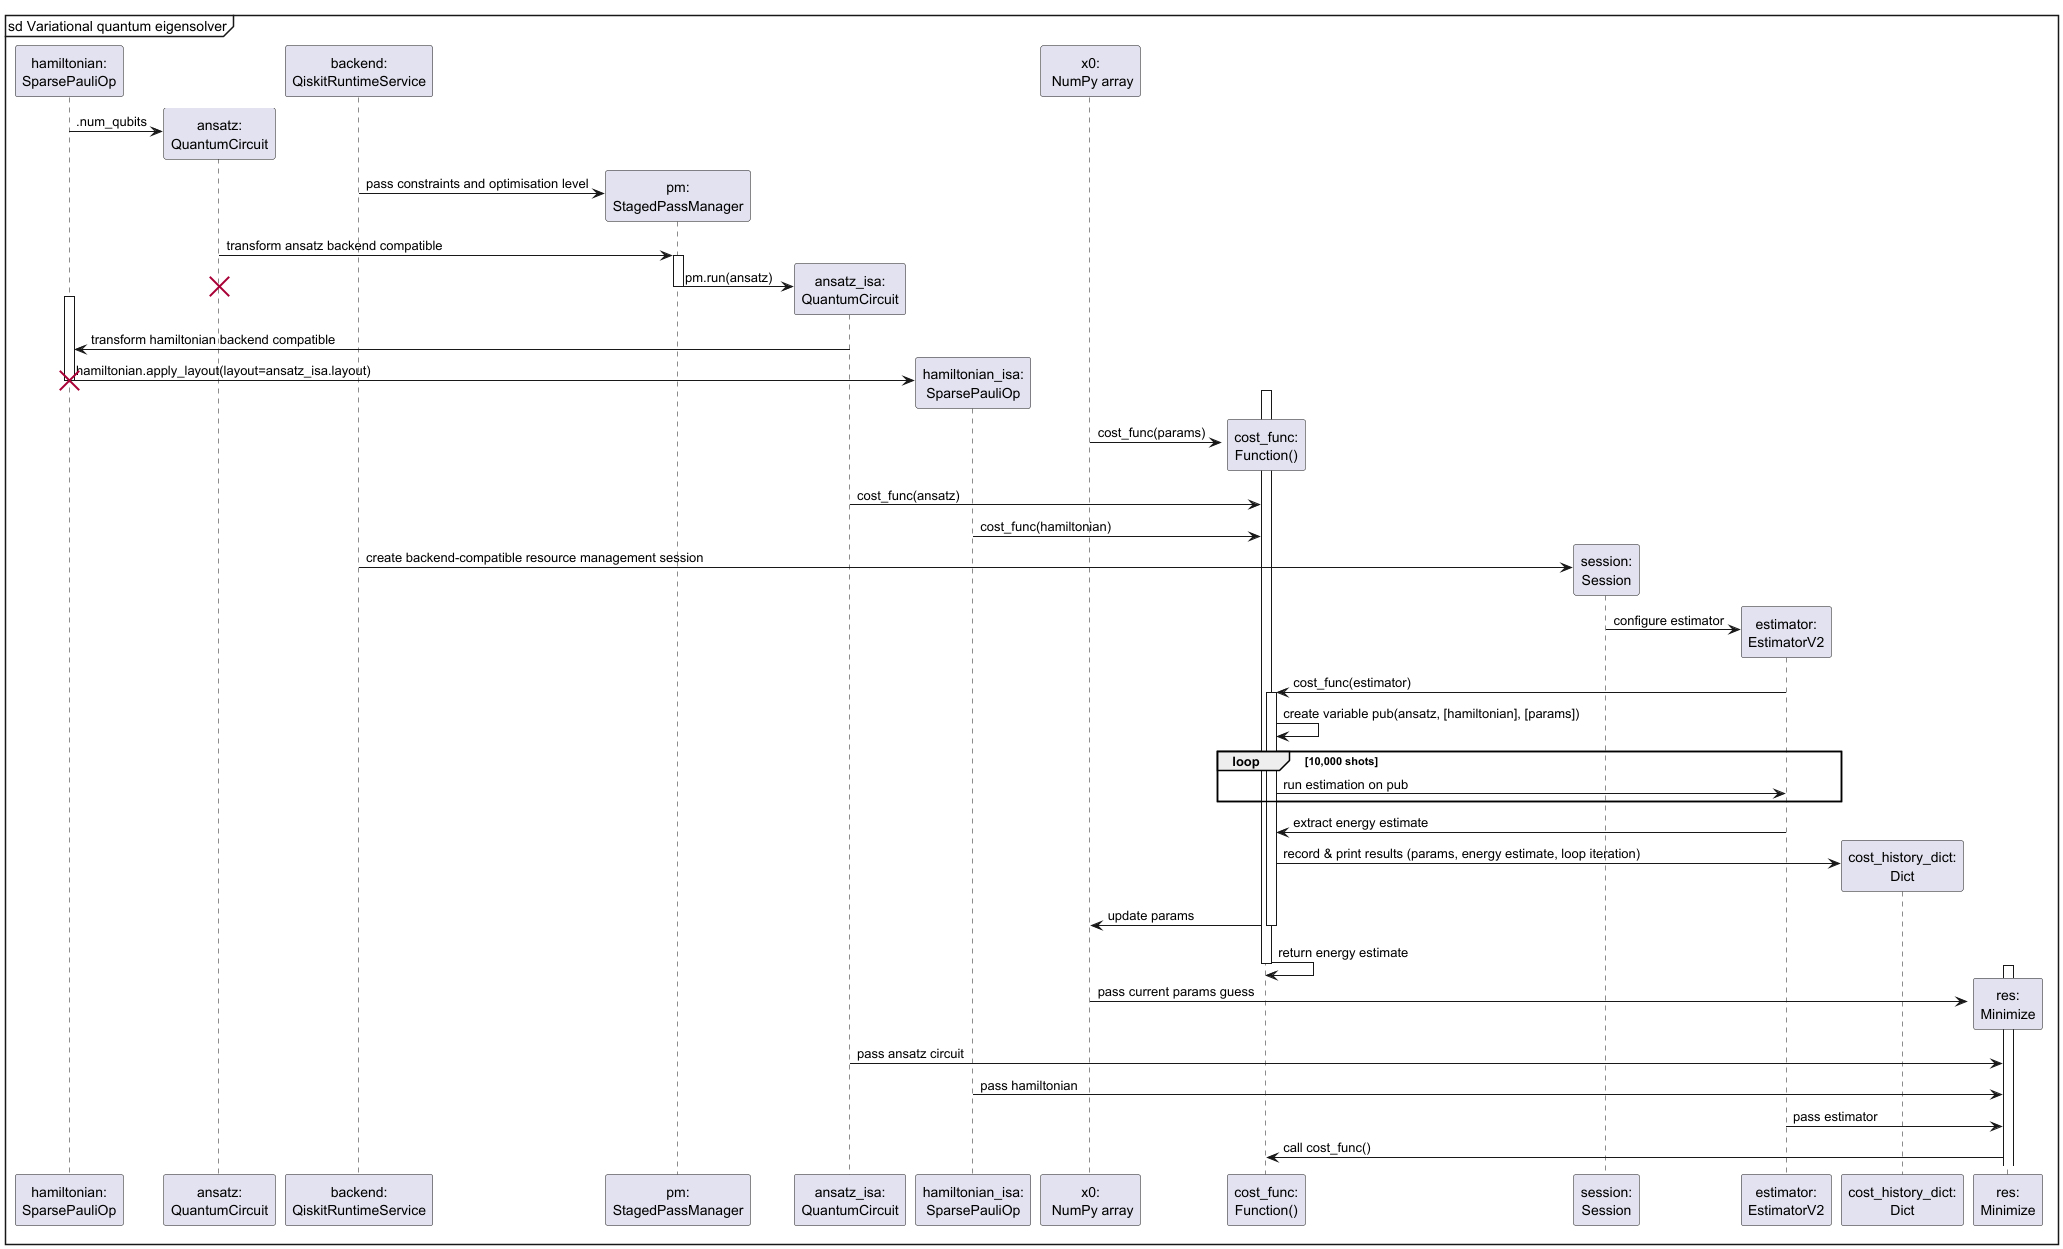
\includegraphics[width=1\linewidth]{vqe_quml_sd_v1.png}
    \caption{First version of the VQE sequence diagram in PUML.}
    \label{fig:vqe_quml_sd_v1}
\end{figure}

\begin{figure}[H]
    \centering
    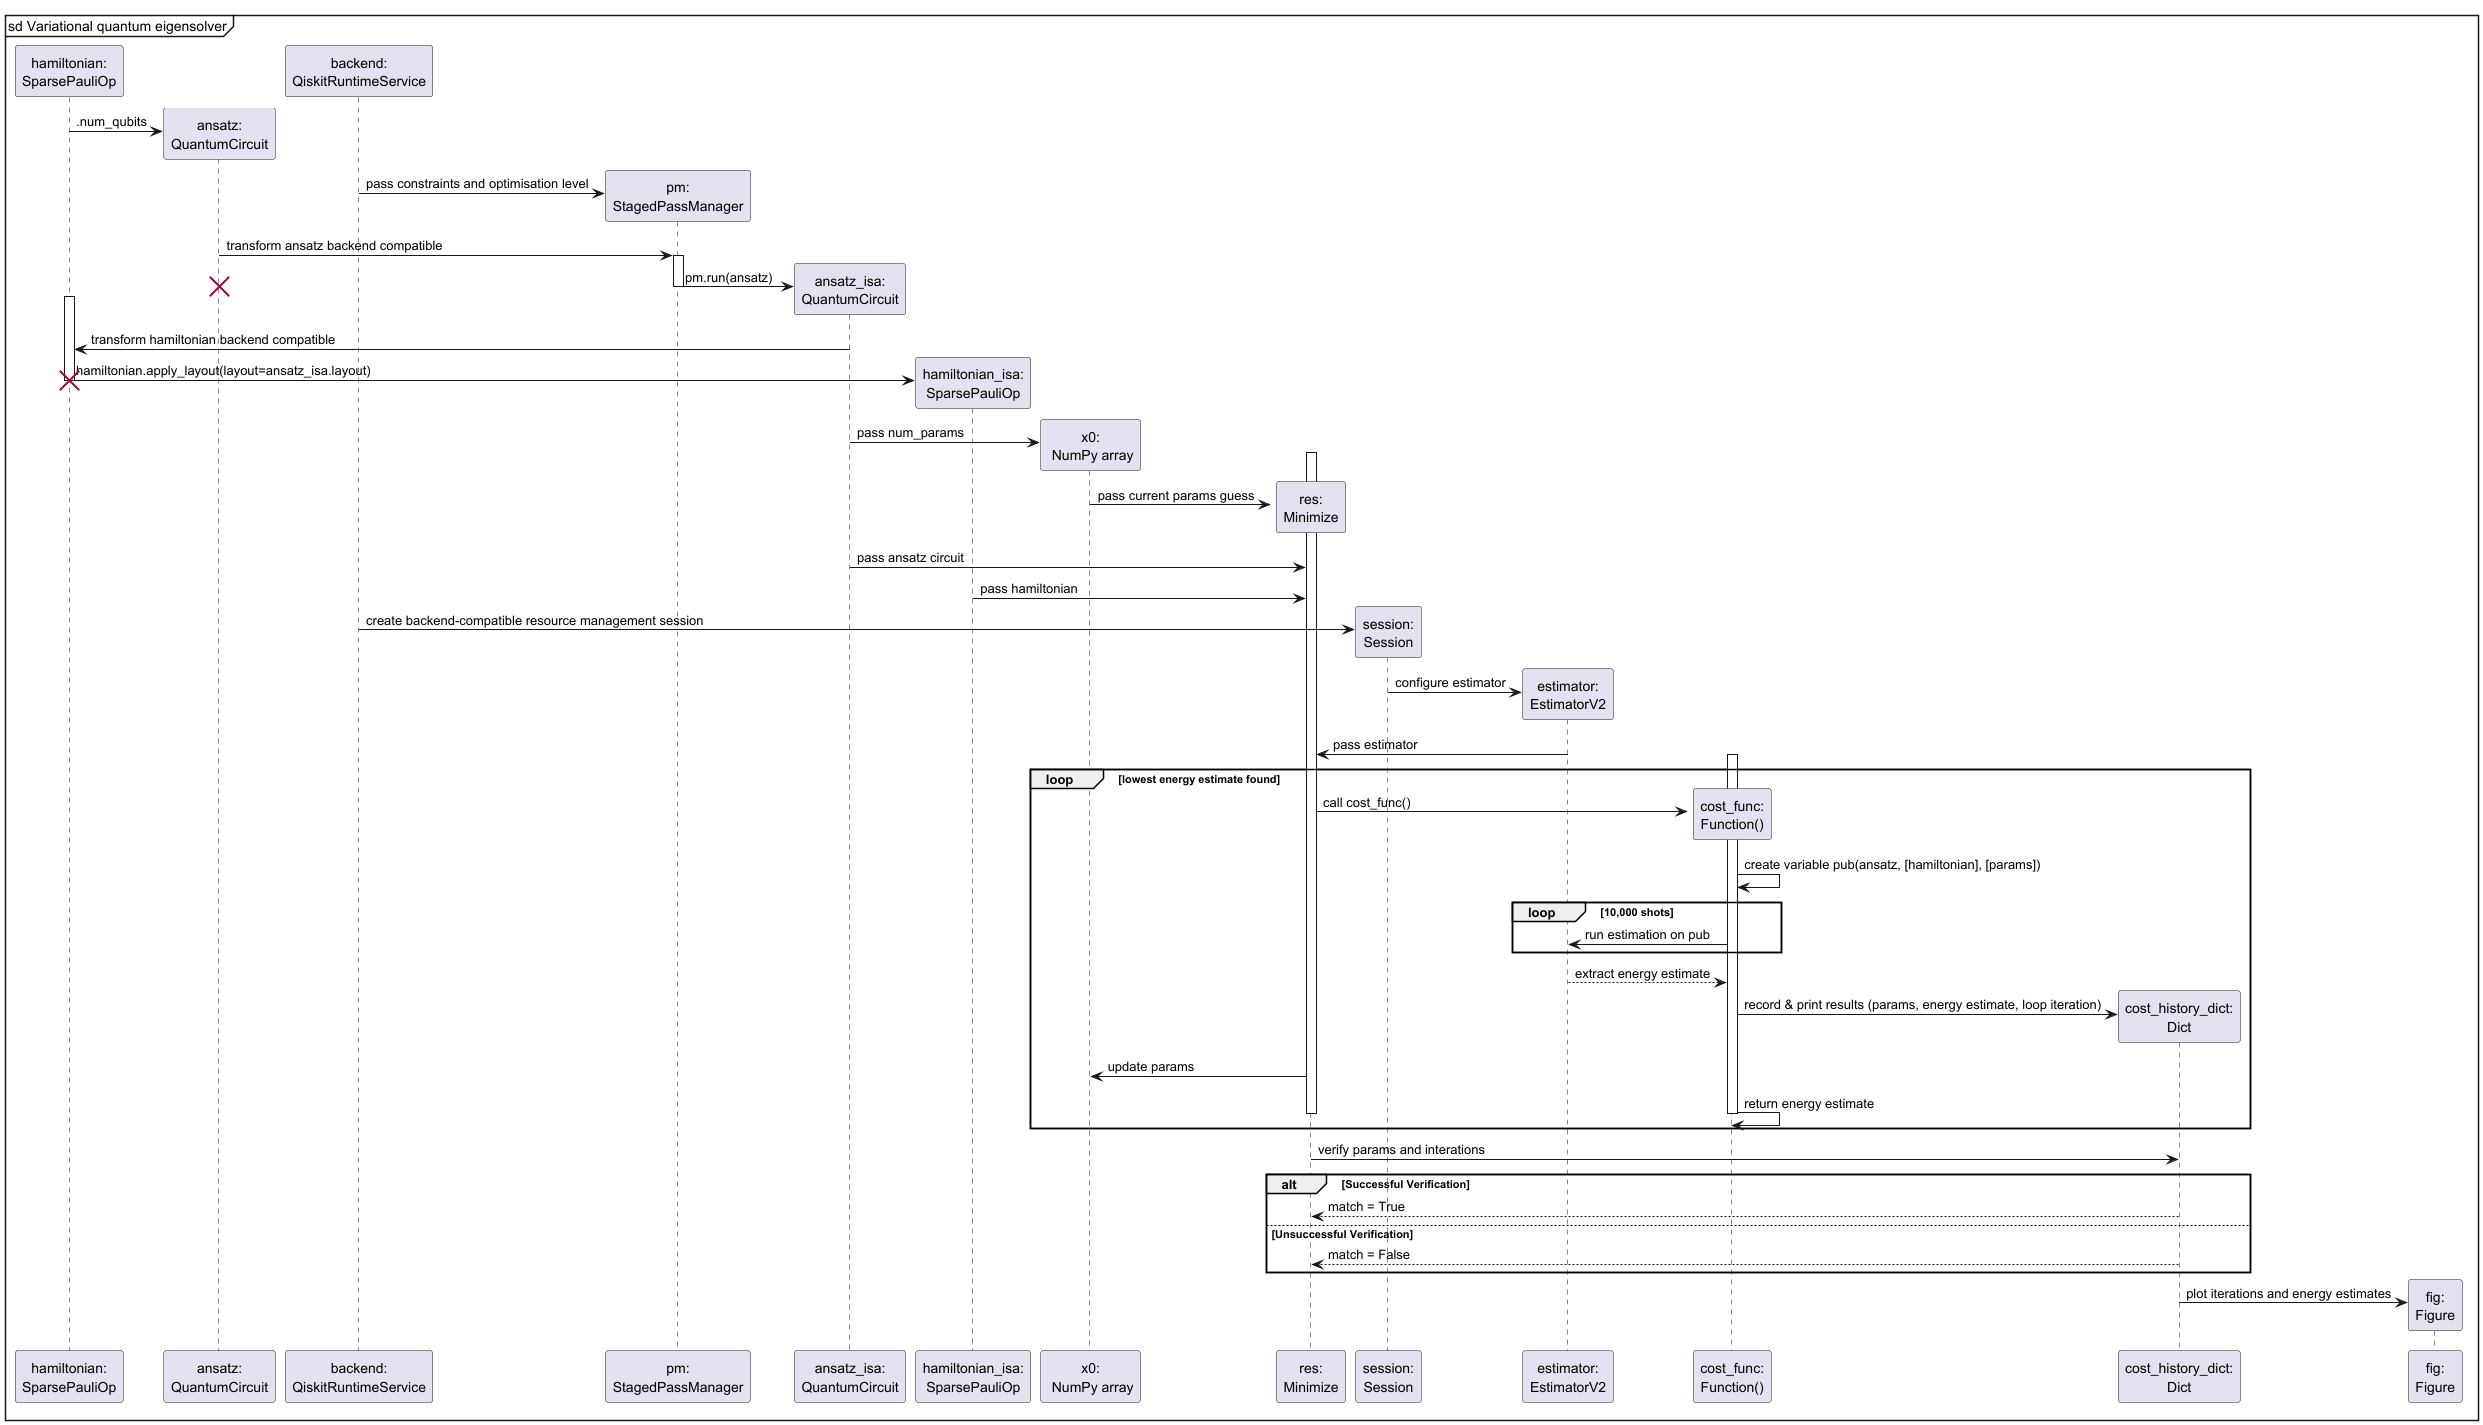
\includegraphics[width=1\linewidth]{vqe_quml_sd_v2.png}
    \caption{Second version of the VQE sequence diagram in PUML, expanding on loop and alt fragments.}
    \label{fig:vqe_quml_sd_v2}
\end{figure}

\begin{figure}[H]
    \centering
    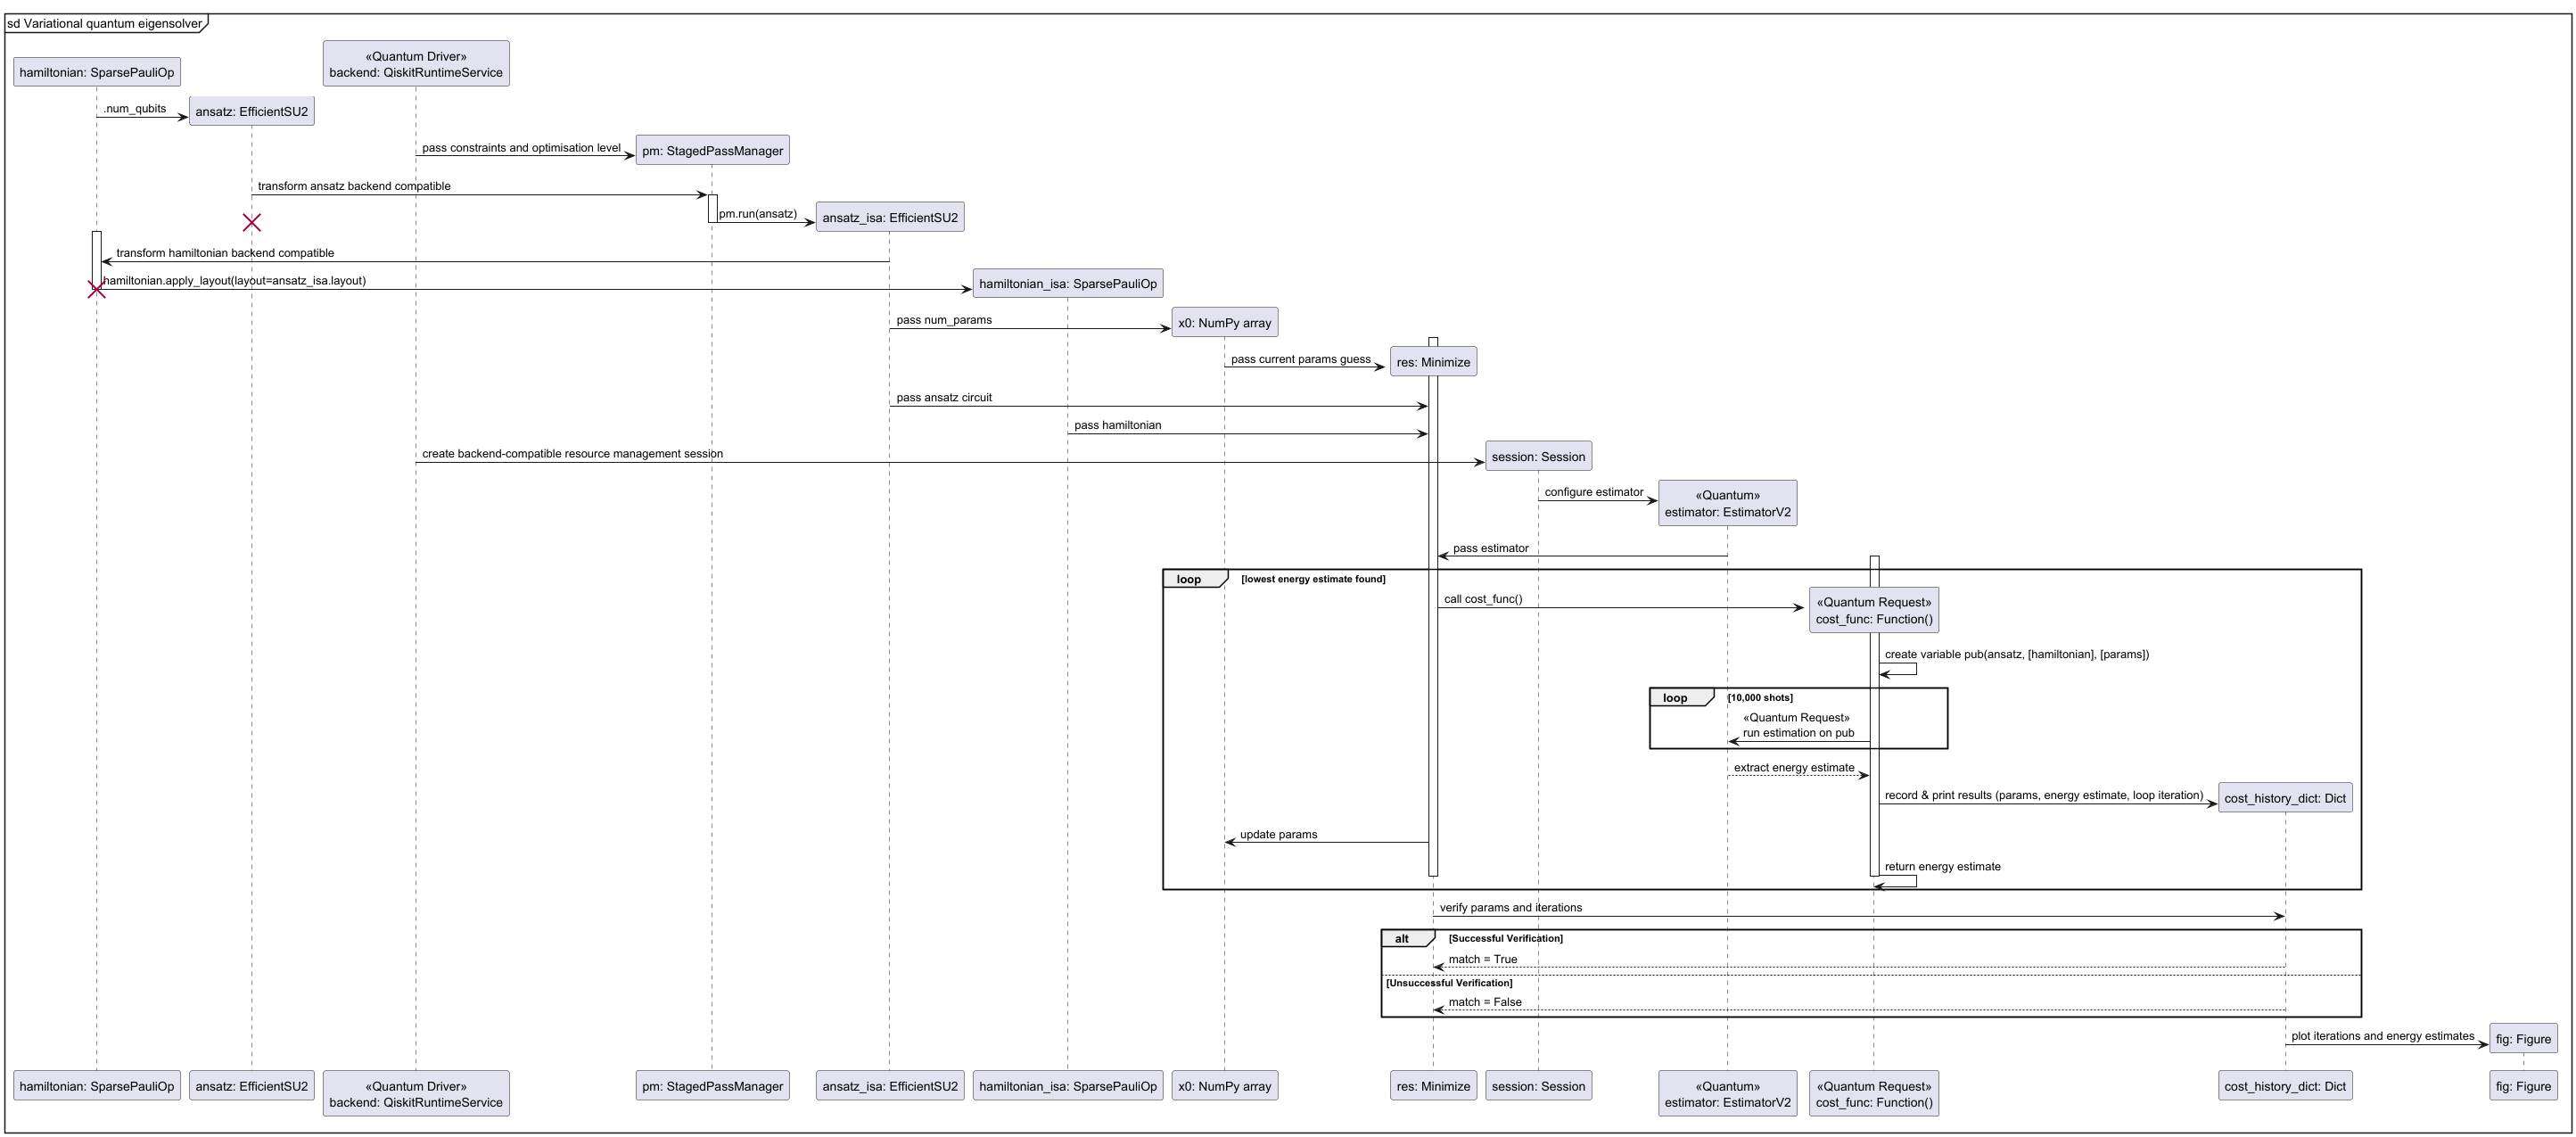
\includegraphics[width=1\linewidth]{vqe_uml_profile_sd_v1.png}
    \caption{Modifying the PUML VQE sequence diagram to incorporate the quantum UML profile's stereotype tags.}
    \label{fig:vqe_uml_profile_sd_v1}
\end{figure}

\begin{figure}[H]
    \centering
    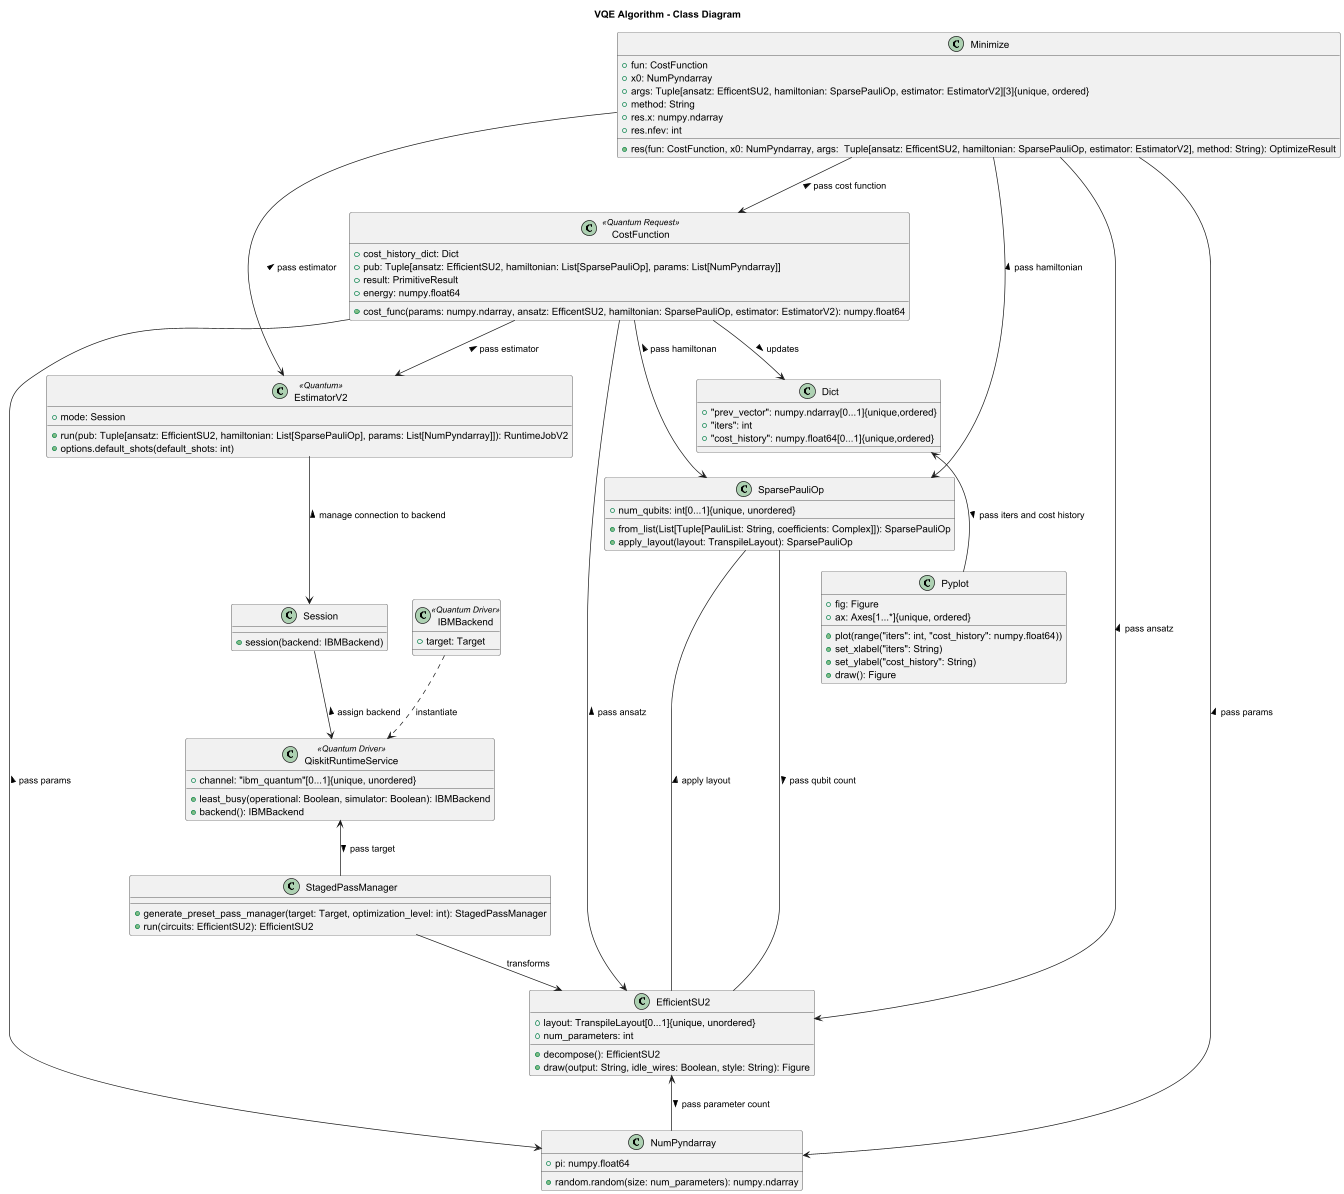
\includegraphics[width=1\linewidth]{vqe_uml_profile_cd_v1-VQE_Algorithm___Class_Diagram.png}
    \caption{Modelling the complete VQE system as a class diagram in PUML using the quantum UML profile stereotypes. Issues with the diagram's comprehensibility are apparent. Incorrect use of reading direction employed at this stage.}
    \label{fig:vqe_uml_profile_cd_v1-VQE_Algorithm___Class_Diagram}
\end{figure}

\begin{figure}[H]
    \centering
    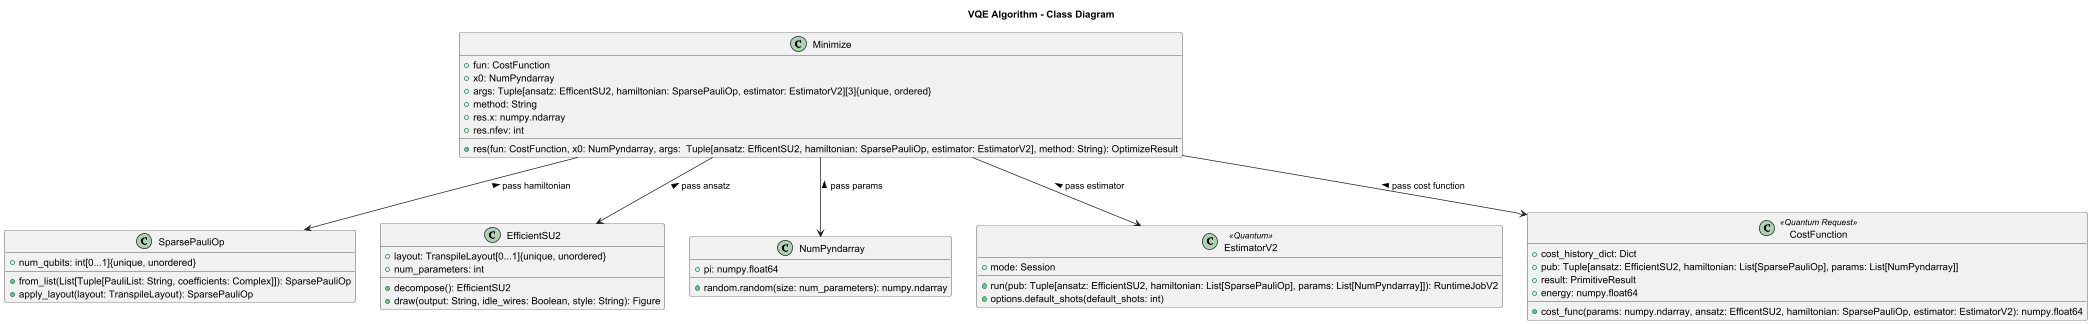
\includegraphics[width=1\linewidth]{vqe_uml_profile_cd_v2-VQE_Algorithm___Class_Diagram.png}
    \caption{Modelling a section of the VQE class diagram in PUML with quantum UML profile stereotypes, the class \textbf{Minimize} being modelled separately.}
    \label{fig:vqe_uml_profile_cd_v2-VQE_Algorithm___Class_Diagram}
\end{figure}

\begin{figure}[H]
    \centering
    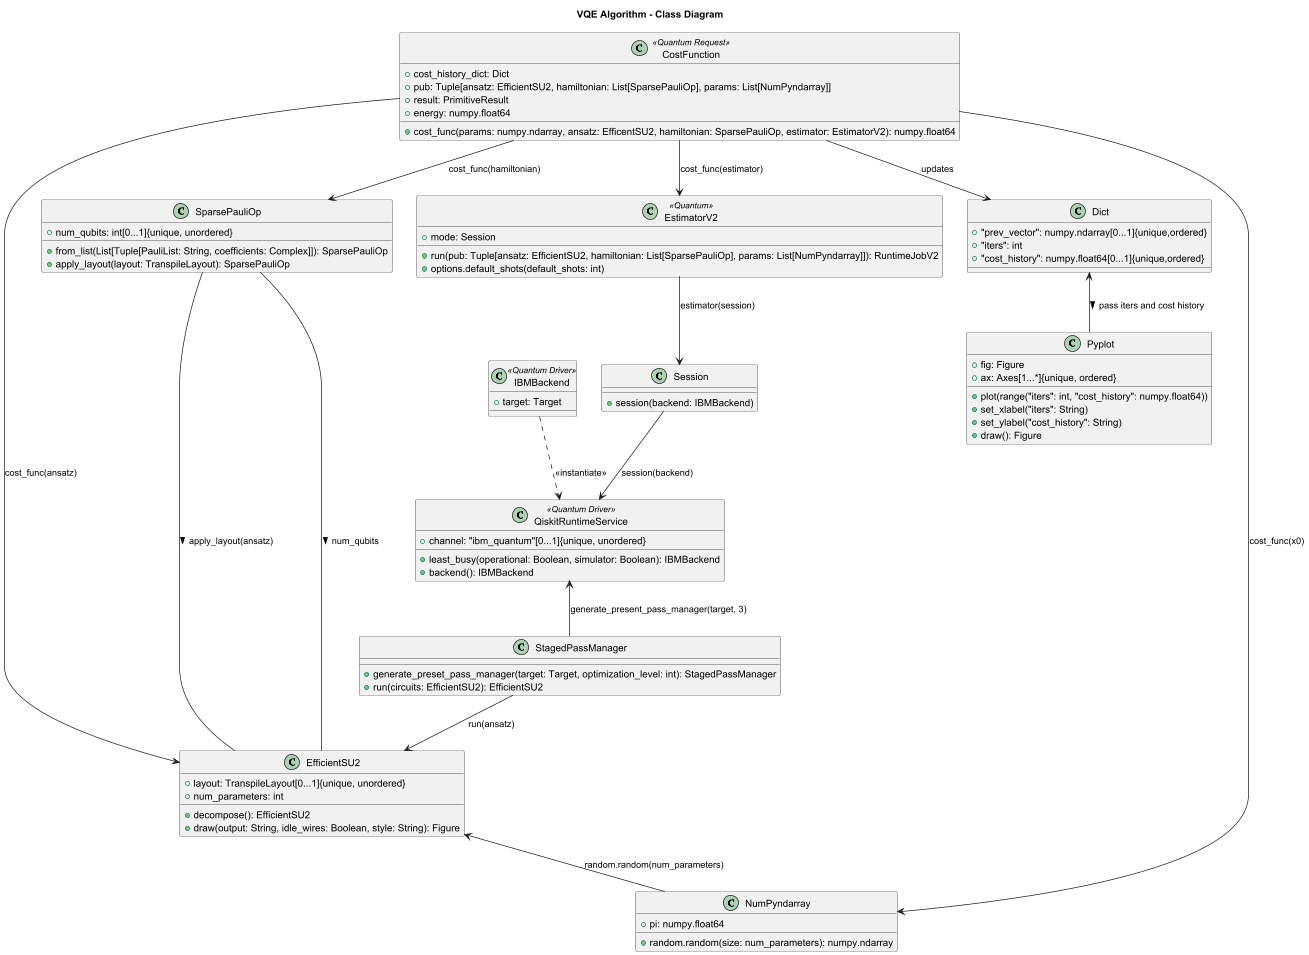
\includegraphics[width=1\linewidth]{vqe_uml_profile_cd_v3-VQE_Algorithm___Class_Diagram.png}
    \caption{Modelling a section of the VQE class diagram in PUML with quantum UML profile stereotypes, the class \textbf{CostFunction} being modelled separately.}
    \label{fig:vqe_uml_profile_cd_v3-VQE_Algorithm___Class_Diagram}
\end{figure}

\begin{figure}[H]
    \centering
    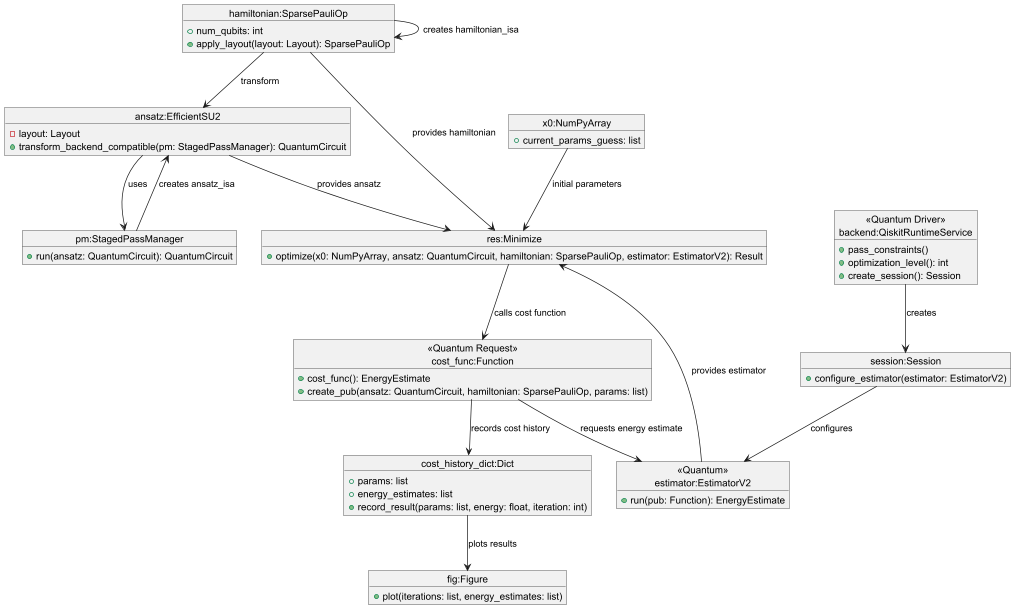
\includegraphics[width=1\linewidth]{vqe_uml_profile_od_v1.png}
    \caption{Exploration of the quantum UML profile modelling VQE as an object diagram in PUML. Considerations were made at the time to elect this instead of a class diagram, but they were dropped.}
    \label{fig:vqe_uml_profile_od_v1}
\end{figure}

\subsection{Mermaid Diagram}

Below is the class diagram generated using Mermaid, which was created to evaluate whether this method would yield more coherent diagrams than PlantUML. The script for this diagram can be found in the GitHub repository linked to this paper\cite{ellygithub}.

\begin{figure}[H]
    \centering
    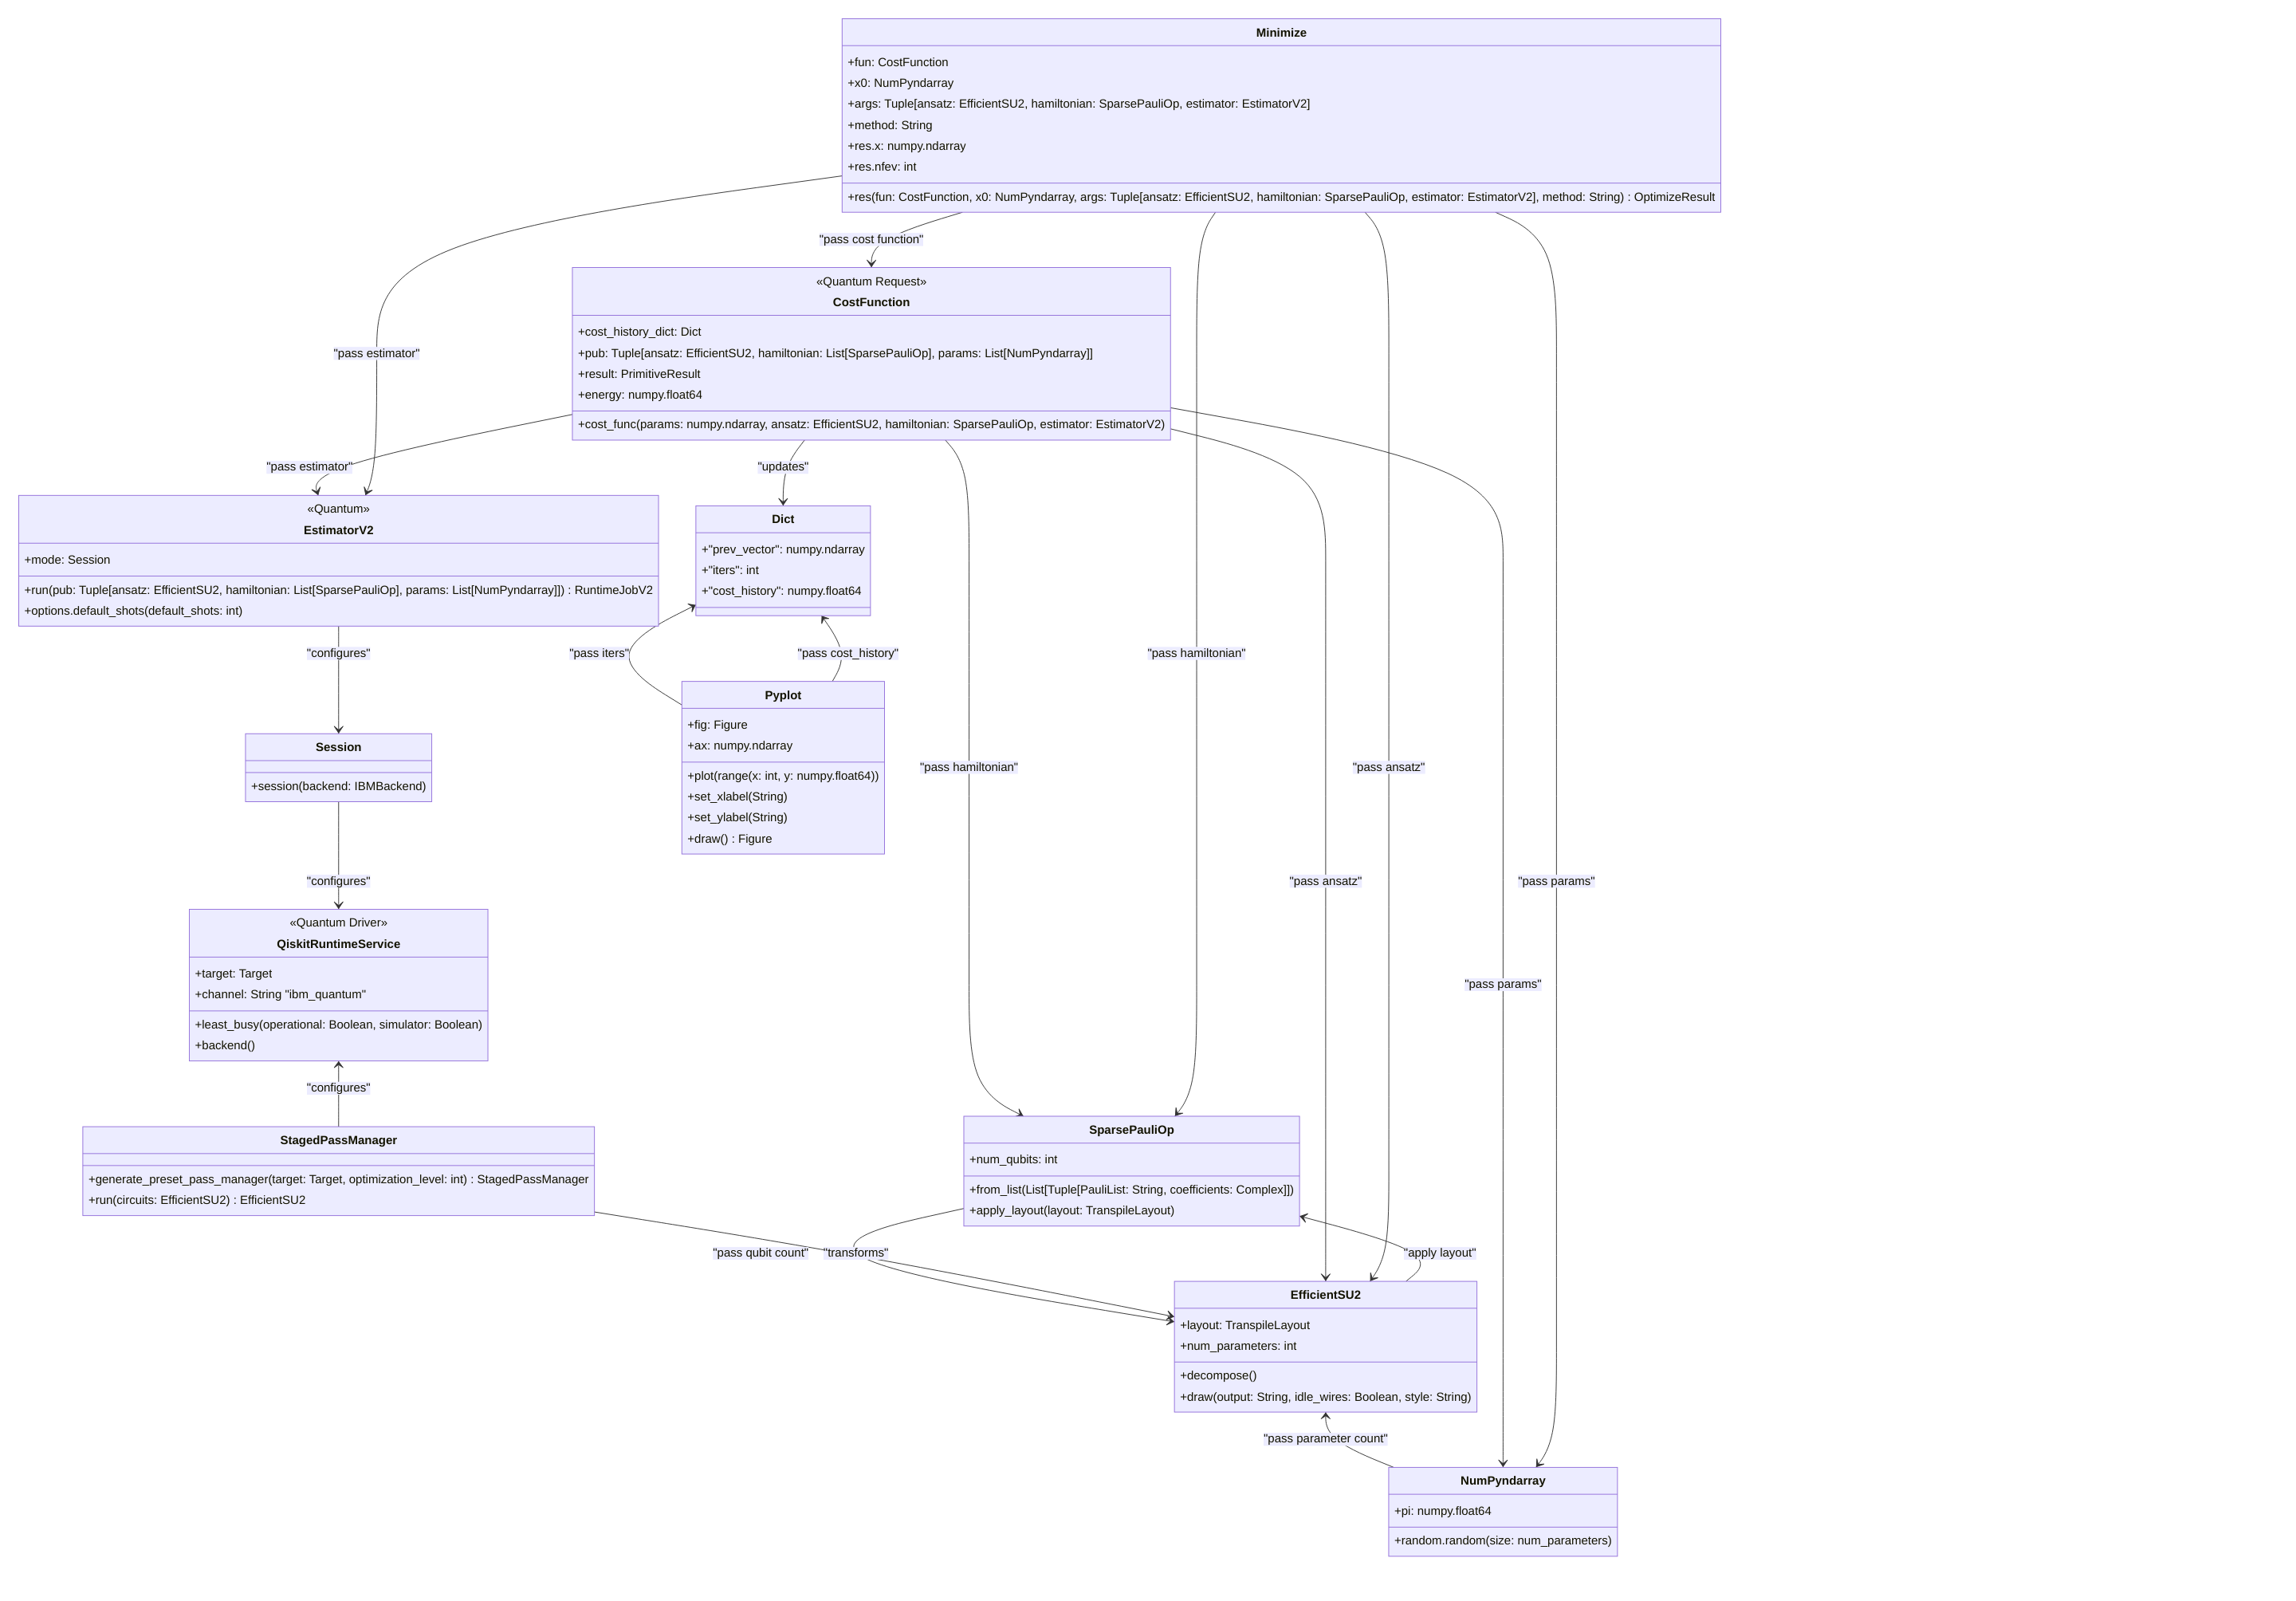
\includegraphics[width=1\linewidth]{mermaidClassDiagram.png}
    \caption{VQE class diagram created using Mermaid. The design remains as convoluted as with PUML, highlighting scalability issues with text-to-diagram tools.}
    \label{fig:mermaidClassDiagram}
\end{figure}

\end{document}
